%---------------------------------------------------------------
\chapter{\babTiga}
%---------------------------------------------------------------

%-----------------------------------------------------------------------------%
\section{Sistem Arsitektur}
%-----------------------------------------------------------------------------%

Perancangan sistem arsitektur aplikasi sistem pengawakan jabatan struktural dapat dilihat pada \textbf{Gambar 3.1.} berikut: 

\begin{figure}
	\centering
	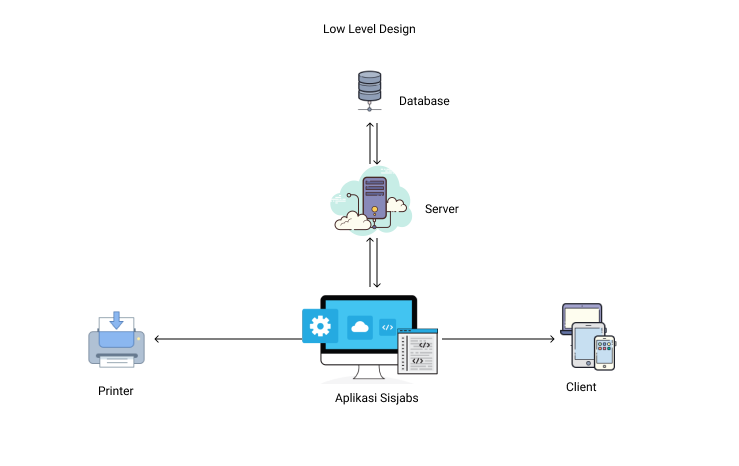
\includegraphics[width=1\textwidth]
	{pics/LowLevelDiagram.png}
	\caption{\textit{Low Level Design}}
	\label{fig:31}
\end{figure}


\subsection{Gambaran Umum Sistem}

Aplikasi "\textbf{SiPJabS : Sistem Pengawakan Jabatan Struktural di Univertias Telkom}" merupakan aplikasi berbasis web yang memudahkan bagi perusahaan dalam pencarian seorang kandidat atau posisi yang kosong. Dalam pembuatan aplikasi ini dibutuhkan fitur \textit{filtering} yang digunakan untuk pencarian kandidat baru, yang sesuai dengan ketentuan yang sudah ditetapkan oleh perusahaan. Sistem \textit{filtering} dapat dilakukan setiap saat, untuk menggantikan pekerjaan lama yang telah berhenti dikarenakan pensiun, meninggal, mengundurkan diri atau diberhentikan karena suatu kebijakan tertentu. \\

Data-data pegawai yang berada di Universitas Telkom dapat dilihat dan data tersebut bersifat rahasia. Sehingga aplikasi ”\textbf{SiPJabS : Sistem Pengawakan Jabatan Struktural di Universitas Telkom}” hanya dapat diakses oleh orang tertentu. Aplikasi ini terdapat satu \textit{user} yang dapat mengelola proses \textit{filtering} dan satu \textit{admin} yang mengelola infrastruktur \textit{database} dan proyek \textit{server} serta jaringan.  

Sistem \textit{filtering} pada apliaksi ini terbagi menjadi dua bagian, yang pertama merupakan \textit{fitering} secara umum dengan isi \textit{form} seperti jabatan minimal dan masa kerja. Yang kedua merupakan \textit{filtering} secara khusus, dimana \textit{user} dapat mencari kandidat dengan syarat yang lebih spesifik lagi untuk dijadikan pilihan, kemudian akan terdapat beberapa nama kandidat, apabila sudah menentukan pilihan dapat menekan tombol \textit{button} pada nama yang akan dipilih dan akan masuk dalam \textit{cart} kandidat.

Apabila proses pencarian kandidat sudah ditemukan dengan salah satu proses \textit{filtering} yang sudah dijelaskan diatas maka, proses selanjutnya akan masuk dalam pembuatan berita acara dan dapat dicetak berupa file pdf.  

\subsection{Target Pengguna Aplikasi}

Aplikasi \textbf{SiPJabS} memiliki beberapa target pengguna diantaranya sebagai berikut:

\begin{enumerate}
\item \textit{User} \\
\textit{User} merupakan pegawai Direktorat Sumber Daya Manusia Universitas Telkom yang membutuhkan kandidat dengan proses \textit{filtering} untuk mengisi posisi yang kosong atau digantikan.

\item \textit{Admin} \\
\textit{Admin} merupakan pegawai Direktorat Pusat Teknologi Informasi Universitas Telkom yang mengelola dan menyediakan data untuk proses filtering.
\end{enumerate}

\subsection{Spesifikasi Target Perangkat}

Spesifikasi dari target perangkat untuk mengakses aplikasi \textbf{SiPJabS} adalah sebagai berikut: 

\begin{enumerate}

\item Komputer atau laptop yang terhubung dengan koneksi internet dan dapat membuka web \textit{browser}.

\item	\textit{Smartphone} atau tablet yang terhubung dengan koneksi internet dan dapat membuka web \textit{browser}.
\end{enumerate}

\subsection{Diagram Alir Aplikasi}

Dalam membangun aplikasi \textbf{SiPJabS}, dibutuhkan diagram alir untuk membantu \textit{developer} dan pengguna dalam memahami sistem yang akan dibuat. Berikut merupakan \textit{flowchart}:

\begin{figure}
	\centering
	\includegraphics[width=1\textwidth]
	{pics/diagram/flowchart.png}
	\caption{\textit{Flowchart}}
	\label{fig:31}
\end{figure}

Lorem ipsum dolor sit amet, consectetuer adipiscing elit. Etiam lobortis facilisis sem.  Nullam nec mi et neque pharetra sollicitudin.  Praesent imperdiet  mi nec ante. Donec ullamcorper, felis non sodales commodo, lectus velit ultrices augue, a dignissim nibh lectus placerat pede. Vivamus nunc nunc, molestie ut, ultricies vel, semper in, velit. Ut porttitor. Praesent in sapien. Lorem ipsum dolor sit amet, consectetuer adipiscing elit. Duis fringilla tristique neque. Sed interdum libero ut metus. Pellentesque placerat.  Nam rutrum augue a leo.  

\newpage
%-----------------------------------------------------------------------------%
\section{Kebutuhan Pengembangan Sistem}
%-----------------------------------------------------------------------------%

Dalam membangun aplikasi \textbf{SiPJabS}, dibutuhkan beberapa perangkat untuk mengimplementasikannya. Perangkat tersebut dibagi menjadi tiga, yaitu perangkat keras (\textit{hardware}), perangkat lunak (\textit{software}) dan Perangkat \textit{server}/\textit{hosting}. Adapun kebutuhan pengembangan sistem adalah sebagai berikut: 

\subsection{Kubutuhan Perangkat Keras (\textit{Hardware}) }

\textit{Hardware} yang dibutuhkan dalam perancangan dan pembuatan aplikasi SiPJabs
adalah sebagai berikut :


\begin{table}[H]
	\centering
	\caption{Tabel Kebutuhan \textit{Hardware}}
	\begin{tabular}{ | c | l | p{75mm} | }
		\hline
		No. & Perangkat Keras & Spesifikasi \\
		\hline
		\multirow{6}{*}{1} & \multirow{6}{*}{Laptop MSI GL62M} & \textit{Processor} : Intel Core i7-7700HQ \\
		& & \textit{Operating System} : Windows 10 Education \\
		& & RAM : 8 GB \\
		& & \textit{Storage} : 128 GB SSD + 1 TB Hardisk \\
		& & \textit{Graphics Card} :  nVidia Geforce GTX 1050 \\
		& & \textit{Display} : 15.6" FHD, Anti-Glare (1920 x 1080) \\
		
		
		\hline
		
		\multirow{6}{*}{2} & \multirow{6}{*}{Laptop HP Pavilion x360} & \textit{Processor} : Intel Core i3-6100U \\
		& & \textit{Operating System} : Windows 10 Home \\
		& & RAM : 12 GB \\
		& & \textit{Storage} : 500 GB Hardisk\\
		& & \textit{Graphics Card} : Intel HD 520 Graphics \\
		& & \textit{Display} : 13.3" HD, Touch Screen \\
		
		\hline
	\end{tabular}
\end{table}


\newpage
\subsection{Kebutuhkan Perangkat Lunak (\textit{Software})}

\textit{Software} yang dibutuhkan dalam perancangan dan pembuatan aplikasi \textbf{SiPJabs}
adalah sebagai berikut:

\begin{table}[H]
	\centering
	\caption{Tabel Kebutuhan \textit{Software}}
	\begin{tabular}{ | c | l | p{64.5mm} | }
		\hline
		No. & Perangkat Lunak & Kegunaan \\
		\hline
		
		1 & Visual Studio Code & \textit{Text editor} untuk menuliskan \textit{coding} aplikasi \\
				
		\hline
		
		2 & XAMPP & Sebagai \textit{server} yang berdiri sendiri, yang terdiri atas program \textit{Apache} HTTP \textit{Server}, MySQL \textit{database}, dan penerjemah bahasa yang ditulis dengan bahasa pemrograman PHP dan Perl \\
		
		\hline
		
		3 & IBM Rational System Architect  & Sebuah \textit{software} untuk mendesain rancangan sistem aplikasi \\
		
		\hline
		
		4 & Figma & Untuk mendesai \textit{user interface} secara online \\
		
		
		\hline
		
		5 & Microsoft Office Word & Untuk membuat dokumen dan laporan \\
		
		\hline
		
		6 & TexStudio & Untuk membuat laporan dalam latex \\
		
		\hline
		
		7 & Adobe Premier Pro & Editing vidio demo dan vidio promosi \\
		
		\hline
		
		8 & Brave dan Mozila Firefox & Web \textit{browser} \\
		
		\hline
	\end{tabular}
\end{table}

\subsection{Kebutuhan \textit{Hosting}}

\textit{Hosting} yang dibutuhkan dalam perancangan dan pembuatan aplikasi\textbf{ SiPJabs}
adalah sebagai berikut :

\begin{table}[H]
	\centering
	\caption{Tabel Kebutuhan \textit{Hosting}}
	\begin{tabular}{ | c |  p{54mm} | p{64mm} | }
		\hline
		No. & Server & Spesifikasi \\
		\hline
		\multirow{5}{*}{1} & \multirow{5}{*}{Server Indonesia} & \textit{Storage} : 2 GB \\
		& & RAM : 1 GB \\
		& & \textit{Bandwith} : Unlimited \\
		& & \textit{Processor} : 1 Core \\
		& & \textit{Domain} : my.id  \\
	
		\hline
	\end{tabular}
\end{table}

%-----------------------------------------------------------------------------%
\section{Perancangan Model Program}
%-----------------------------------------------------------------------------%
Perancangan model program dalam pembuatan aplikasi \textit{SiPJabS} antara
lain \textit{Use Case Diagram}, \textit{Use Case Scenario}, \textit{Class Diagram},
\textit{Entity Relationship Diagram} (ERD). Adapun perancangan model program adalah sebagai berikut :

\subsection{Use Case Diagram}

\begin{figure}
	\centering
	\includegraphics[width=1\textwidth]
	{pics/diagram/usecase.png}
	\caption{\textbf{Use Case Diagram}}
	\label{fig:32}
\end{figure}

Lorem ipsum dolor sit amet, consectetuer adipiscing elit. Etiam lobortis facilisis sem.  Nullam nec mi et neque pharetra sollicitudin.  Praesent imperdiet  mi nec ante. Donec ullamcorper, felis non sodales commodo, lectus velit ultrices augue, a dignissim nibh lectus placerat pede. Vivamus nunc nunc, molestie ut, ultricies vel, semper in, velit. Ut porttitor. Praesent in sapien. Lorem ipsum dolor sit amet, consectetuer adipiscing elit. Duis fringilla tristique neque. Sed interdum libero ut metus. Pellentesque placerat.  Nam rutrum augue a leo.  

\subsection{Use Case Skenario}
Berikut merupakan \textit{use case scenario} dalam pembuatan aplikasi SiPJabS:

\begin{enumerate}
	\item Skenario \textit{Login}
	
	Nomor \kern 3.6pc : SP-01 \\
	Nama Use Case : Melakukan \textit{login} \\
	Aktor \kern 4.1 pc : \textit{Admin} \\
	Tipe \kern 4.6pc : \textit{Primary} \\
	Tujuan \kern 3.6pc : \textit{Admin} dapat menggunakan aplikasi \\
	Deskripsi \kern 2.5pc : 
	
	\begin{itemize}
		\item \textit{Admin} menginputkan \textit{username} dan \textit{password}
		\item Sistem akan mencocokkan data
		\item Sistem menampilkan halaman utama aplikasi
	\end{itemize}

	\begin{table}
		\caption{Skenario \textit{Login}}
		\centering
		\begin{tabular}{ | p{60mm} | p{68mm} |}
			\hline 
			\textbf{Aktor} & \textbf{Sistem} \\
			\hline
			
			1.	Menginputkan \textit{username} dan \textit{password} &  \\
			
			\hline
			
			& 2. Mencocokkan data \\
			
			\hline
			
			& 3.	Menampilkan halaman utama aplikasi \\
		
			\hline
			
		\end{tabular}
	\end{table}

\item Skenario\textit{ Edit Profile}

Nomor \kern 3.6pc : SP-02 \\
Nama Use Case : Melakukan \textit{edit profile} \\
Aktor \kern 4.1 pc : \textit{Admin} \\
Tipe \kern 4.6pc : \textit{Primary} \\
Tujuan \kern 3.6pc : \textit{Admin} dapat melakukan \textit{edit} pada \textit{profile} \\
Deskripsi \kern 2.5pc : 

\begin{itemize}
	\item \textit{Admin} menuju ke halaman \textit{profile}
	\item Sistem akan menampilkan halaman \textit{profile}
	\item \textit{Admin} memilih \textit{edit profile}
	\item Sistem menampilkan \textit{pop-up form edit profile}
	\item \textit{Admin} menginputkan data
	
\end{itemize}

\begin{table}
	\caption{Skenario \textit{Edit Profile}}
	\centering
	\begin{tabular}{ |  p{59mm} | l |}
		\hline 
		\textbf{Aktor} & \textbf{Sistem} \\
		\hline
		
		1.	Menuju ke halaman \textit{profile} &  \\
		
		\hline
		
		&  2.	Menampilkan halaman \textit{profile} \\
		
		\hline
		
		 3. Memilih \textit{edit profile} & \\
		
		\hline
		
			& 4.	Menampilkan\textit{ pop-up form edit profile} \\
		
		\hline
		
		5.	Menginputkan data  & \\
		\hline
		
		& 6.	Menyimpan data perubahan\\
		\hline
		
	\end{tabular}
\end{table}

\item Skenario \textit{Reset Password}

Nomor \kern 3.6pc : SP-03 \\
Nama Use Case : Melakukan \textit{reset password} \\
Aktor \kern 4.1 pc : \textit{Admin} \\
Tipe \kern 4.6pc : \textit{Primary} \\
Tujuan \kern 3.6pc : \textit{Admin} dapat melakukan \textit{reset password} pada \textit{profile} \\
Deskripsi \kern 2.5pc : 

\begin{itemize}
	\item \textit{Admin} menuju ke halaman \textit{profile}
	\item Sistem akan menampilkan halaman \textit{profile}
	\item \textit{Admin} memilih\textit{ reset password}
	\item Sistem menampilkan \textit{pop-up reset password}
	\item \textit{Admin} menginputkan \textit{password} lama dan baru
	\item Sistem menyimpan data perubahan
	
\end{itemize}

\begin{table}
	\caption{Skenario \textit{Reset Password}}
	\centering
	\begin{tabular}{ |  p{61mm} | l |}
		\hline 
		\textbf{Aktor} & \textbf{Sistem} \\
		\hline
		
		1.	Menuju ke halaman \textit{profile} &  \\
		
		\hline
		
		&  2.	Menampilkan halaman \textit{profile} \\
		
		\hline
		
		3. Memilih \textit{reset password} & \\
		
		\hline
		
		& 4.	Menampilkan\textit{ pop-up reset password} \\
		
		\hline
		
		5.	Menginputkan \textit{password} lama dan baru  & \\
		\hline
		
		
		& 6.	Menyimpan data perubahan \\
		\hline
		
	\end{tabular}
\end{table}

\newpage

\item Skenario Tambah \textit{Users}

Nomor \kern 3.6pc : SP-04 \\
Nama Use Case : Menambahkan \textit{users} \\
Aktor \kern 4.1 pc : \textit{Admin} \\
Tipe \kern 4.6pc : \textit{Primary} \\
Tujuan \kern 3.6pc : \textit{Admin} dapat menambahkan \textit{users} \\
Deskripsi \kern 2.5pc : 

\begin{itemize}
	\item \textit{Admin} menuju ke halaman data \textit{users}
	\item Sistem akan menampilkan halaman data \textit{users}
	\item \textit{Admin} memilih tambah \textit{users}
	\item Sistem menampilkan halaman \textit{form} tambah \textit{users}
	\item \textit{Admin} menginputkan data
	\item Sistem menyimpan data
	\item Sistem menampilkan \textit{pop-up} tanda berhasil menambahkan \textit{users}
	
\end{itemize}

\begin{table}
	\caption{Skenario Tambah \textit{Users}}
	\centering
	\begin{tabular}{ | l | p{72mm} |}
		\hline 
		\textbf{Aktor} & \textbf{Sistem} \\
		\hline
		
		1.	Menuju ke halaman data \textit{users} &  \\
		
		\hline
		
		&  2. Menampilkan halaman data \textit{users} \\
		
		\hline
		
		3. Memilih tambah \textit{users} & \\
		
		\hline
		
		& 4. Menampilkan halaman form tambah \textit{users} \\
		
		\hline
		
		5.	Menginputkan data  & \\
		\hline
		
		
		& 6.	Menyimpan data \\
		\hline
		
		& 7. Menampilkan \textit{pop-up} tanda berhasil menambahkan \textit{users} \\
		\hline
		
	\end{tabular}
\end{table}

\newpage
\item Skenario \textit{Edit Users}

Nomor \kern 3.6pc : SP-05 \\
Nama Use Case : Melakukan \textit{edit} data \textit{users} \\
Aktor \kern 4.1 pc : \textit{Admin} \\
Tipe \kern 4.6pc : \textit{Primary} \\
Tujuan \kern 3.6pc : \textit{Admin} dapat meng\textit{edit} data \textit{users} \\
Deskripsi \kern 2.5pc : 

\begin{itemize}
	\item \textit{Admin} menuju ke halaman data \textit{users}
	\item Sistem akan menampilkan halaman data \textit{users}
	\item \textit{Admin} memilih \textit{edit} pada salah satu \textit{users}
	\item Sistem menampilkan \textit{pop-up form edit users}
	\item \textit{Admin} menginputkan data
	\item Sistem menyimpan data perubahan
	\item Sistem menampilkan \textit{pop-up} tanda berhasil mengedit data
	
\end{itemize}

\begin{table}
	\caption{Skenario \textit{Edit Users}}
	\centering
	\begin{tabular}{ | l | p{65mm} |}
		\hline 
		\textbf{Aktor} & \textbf{Sistem} \\
		\hline
		
		1.	Menuju ke halaman data \textit{users} &  \\
		
		\hline
		
		&  2.	Menampilkan halaman data \textit{users} \\
		
		\hline
		
		3. Memilih \textit{edit} pada salah satu \textit{users} & \\
		
		\hline
		
		& 4.	Menampilkan \textit{pop-up form edit users} \\
		
		\hline
		
		5.	Menginputkan data  & \\
		\hline
		
		& 7.	Menyimpan data \\
		\hline
		
		& 8.	Menampilkan \textit{pop-up} tanda berhasil edit \textit{users} \\
		\hline
		
	\end{tabular}
\end{table}

\newpage

\item Skenario \textit{Delete Users}

Nomor \kern 3.6pc : SP-06 \\
Nama Use Case : Melakukan \textit{delete} data \textit{users} \\
Aktor \kern 4.1 pc : \textit{Admin} \\
Tipe \kern 4.6pc : \textit{Primary} \\
Tujuan \kern 3.6pc : \textit{Admin} dapat \textit{delete} data \textit{users} \\
Deskripsi \kern 2.5pc : 

\begin{itemize}
	\item \textit{Admin} menuju ke halaman data \textit{users}
	\item Sistem akan menampilkan halaman data \textit{users}
	\item \textit{Admin} memilih \textit{delete} pada salah satu \textit{users}
	\item Sistem menampilkan \textit{pop-up} tanda berhasil hapus data
	
\end{itemize}

\begin{table}
	\caption{Skenario \textit{Delete Users}}
	\centering
	\begin{tabular}{ | l | p{61mm} |}
		\hline 
		\textbf{Aktor} & \textbf{Sistem} \\
		\hline
		
		1.	Menuju ke halaman data \textit{users} &  \\
		
		\hline
		
		&  2.	Menampilkan halaman data \textit{users} \\
		
		\hline
		
		3. Memilih \textit{delete} pada salah satu \textit{users} & \\
		
		\hline
		
		& 4.	Menampilkan \textit{pop-up} tanda berhasil \textit{delete} data \\
		
		\hline
		
	\end{tabular}
\end{table}

\item Skenario \textit{View} Pegawai

Nomor \kern 3.6pc : SP-07 \\
Nama Use Case : Melakukan \textit{view} data pegawai \\
Aktor \kern 4.1 pc : \textit{Admin} \\
Tipe \kern 4.6pc : \textit{Primary} \\
Tujuan \kern 3.6pc : \textit{Admin} dapat melihat data pegawai \\
Deskripsi \kern 2.5pc : 

\begin{itemize}
	\item Admin menuju ke halaman data pegawai
	\item Sistem akan menampilkan halaman data pegawai
	\item Admin memilih \textit{view} pada salah satu pegawai
	\item Sistem menampilkan \textit{pop-up} detail pegawai
	\item Admin dapat melihat data detail pegawai
	
\end{itemize}

\begin{table}
	\caption{Skenario \textit{View} Pegawai}
	\centering
	\begin{tabular}{ | p{60mm} | p{68mm} |}
		\hline 
		\textbf{Aktor} & \textbf{Sistem} \\
		\hline
		
		1.	Menuju ke halaman data pegawai &  \\
		
		\hline
		
		&  2.	Menampilkan halaman data pegawai \\
		
		\hline
		
		3. Memilih \textit{view} pada salah satu data pegawai & \\
		
		\hline
		
		& 4.	Menampilkan \textit{pop-up} detail pegawai \\
		
		\hline
		
		5.	Melihat data detail pegawai  & \\
		\hline
		
		
	\end{tabular}
\end{table}

\item Skenario Tambah Pegawai

Nomor \kern 3.6pc : SP-08 \\
Nama Use Case : Melakukan tambah data pegawai \\
Aktor \kern 4.1 pc : \textit{Admin} \\
Tipe \kern 4.6pc : \textit{Primary} \\
Tujuan \kern 3.6pc : \textit{Admin} dapat menambahkan data pegawai \\
Deskripsi \kern 2.5pc : 

\begin{itemize}
	\item Admin menuju ke halaman data pegawai
	\item Sistem akan menampilkan halaman data pegawai
	\item Admin memilih tambah data pegawai
	\item Sistem menampilkan form tambah pegawai
	\item Admin menginputkan data
	\item Sistem menyimpan data
	\item Sistem menampilkan pop-up berhasil menambahkan data
	
\end{itemize}

\begin{table}
	\caption{Skenario Tambah Pegawai}
	\centering
	\begin{tabular}{ | l | p{66.5mm} |}
		\hline 
		\textbf{Aktor} & \textbf{Sistem} \\
		\hline
		
		1.	Menuju ke halaman data pegawai &  \\
		
		\hline
		
		&  2.	Menampilkan halaman data pegawai \\
		
		\hline
		
		3. Memilih tambah data pegawai & \\
		
		\hline
		
		& 4.	Menampilkan form tambah pegawai \\
		
		\hline
		
		5. Menginputkan data & \\
		\hline
		
		& 6.	Menyimpan data \\
		
		\hline
		
		& 7.	Menampilkan pop-up berhasil menambahkan data \\
		
		\hline
		
		
	\end{tabular}
\end{table}

\item Skenario \textit{Edit} Pegawai

Nomor \kern 3.6pc : SP-09 \\
Nama Use Case : Melakukan \textit{edit} data pegawai \\
Aktor \kern 4.1 pc : \textit{Admin} \\
Tipe \kern 4.6pc : \textit{Primary} \\
Tujuan \kern 3.6pc : \textit{Admin} dapat mengedit data pegawai \\
Deskripsi \kern 2.5pc : 

\begin{itemize}
	\item Admin menuju ke halaman data pegawai
	\item Sistem akan menampilkan halaman data pegawai
	\item Admin memilih \textit{edit} pada salah satu pegawai
	\item Sistem menampilkan edit data pegawai
	\item Admin menginputkan data
	\item Sistem menyimpan data perubahan
	\item Sistem menampilkan pop-up berhasil merubah data
	
\end{itemize}

\begin{table}
	\caption{Skenario \textit{Edit} Pegawai}
	\centering
	\begin{tabular}{ | p{72mm} | p{56mm} |}
		\hline 
		\textbf{Aktor} & \textbf{Sistem} \\
		\hline
		
		1.	Menuju ke halaman data pegawai &  \\
		
		\hline
		
		&  2.	Menampilkan halaman data pegawai \\
		
		\hline
		
		3. Memilih \textit{edit} pada salah satu pegawai & \\
		
		\hline
		
		& 4.	Menampilkan form edit data pegawai \\
		
		\hline
		
		5.	Menginpputkan data  & \\
		\hline
		
			& 6.	Menyimpan data perubahan \\
		
		\hline
		
		& 7.	Menampilkan pop-up berhasil merubah data \\
		
		\hline
		
		
	\end{tabular}
\end{table}

\newpage

\item Skenario \textit{View} Kandidat

Nomor \kern 3.6pc : SP-10 \\
Nama Use Case : Melakukan \textit{view} data kandidat \\
Aktor \kern 4.1 pc : Admin \\
Tipe \kern 4.6pc : Primary \\
Tujuan \kern 3.6pc : Admin dapat melihat data kandidat \\
Deskripsi \kern 2.5pc : 

\begin{itemize}
	\item Admin menuju ke halaman data kandidat
	\item Sistem akan menampilkan halaman data kandidat
	\item Admin memilih \textit{view} pada salah satu kandidat
	\item Sistem menampilkan pop-up detail data kandidat
	\item Admin dapat melihat data detail kandidat
	
\end{itemize}

\begin{table}
	\caption{Skenario View Kandidat}
	\centering
	\begin{tabular}{ |  p{73mm} | p{55mm} |}
		\hline 
		\textbf{Aktor} & \textbf{Sistem} \\
		\hline
		
		1.	Menuju ke halaman data kandidat &  \\
		
		\hline
		
		&  2.	Menampilkan halaman data kandidat \\
		
		\hline
		
		3. Memilih view pada salah satu kandidat & \\
		
		\hline
		
		& 4.	Menampilkan pop-up detail data kandidat \\
		
		\hline
		
		5. Melihat data detail kandidat  & \\
		\hline
		
		
	\end{tabular}
\end{table}

\item Skenario Print Form Kandidat

Nomor \kern 3.6pc : SP-11 \\
Nama Use Case : Melakukan print form data kandidat \\
Aktor \kern 4.1 pc : Admin \\
Tipe \kern 4.6pc : Primary \\
Tujuan \kern 3.6pc : Admin dapat mencetak form data kandidat \\
Deskripsi \kern 2.5pc : 

\begin{itemize}
	\item Admin menuju ke halaman data kandidat
	\item Sistem akan menampilkan halaman data kandidat
	\item Admin memilih print pdf pada salah satu data kandidat
	
\end{itemize}

\begin{table}
	\caption{Skenario Print Form Kandidat}
	\centering
	\begin{tabular}{ | p{61.5mm} | p{67mm} |}
		\hline 
		\textbf{Aktor} & \textbf{Sistem} \\
		\hline
		
		1.	Menuju ke halaman data kandidat &  \\
		
		\hline
		
		&  2.	Menampilkan halaman data kandidat \\
		
		\hline
		
		3. Memilih print pdf pada salah satu data kandidat & \\
		
		\hline
	
		
	\end{tabular}
\end{table}

\item Skenario Tambah Unit Kerja

Nomor \kern 3.6pc : SP-12 \\
Nama Use Case : Menambahkan data unit kerja \\
Aktor \kern 4.1 pc : Admin \\
Tipe \kern 4.6pc : Primary \\
Tujuan \kern 3.6pc : Admin dapat menambahkan data unit kerja \\
Deskripsi \kern 2.5pc : 

\begin{itemize}
	\item Admin menuju ke halaman data unit kerja
	\item Sistem akan menampilkan halaman data unit kerja
	\item Admin memilih tambah unit kerja
	\item Sistem menampilkan pop-up form tambah unit kerja
	\item Admin menginputkan data
	\item Sistem menyimpan data
	\item Sistem menampilkan pop-up tanda data berhasil ditambahkan
	
\end{itemize}

\begin{table}
	\caption{Skenario Tambah Unit Kerja}
	\centering
	\begin{tabular}{ | l | p{65mm} |}
		\hline 
		\textbf{Aktor} & \textbf{Sistem} \\
		\hline
		
		1.	Menuju ke halaman data unit kerja &  \\
		
		\hline
		
		&  2.	Menampilkan halaman data unit kerja \\
		
		\hline
		
		3. Memilih tambah unit kerja & \\
		
		\hline
		
		& 4.	Menampilkan pop-up form tambah unit kerja \\
		
		\hline
		
		5.	Menginputkan data  & \\
		\hline
		
		& 6.	Menyimpan data \\
		\hline
		
		& 7.	Menampilkan pop-up tanda berhasil menambahkan data \\
		\hline
		
	\end{tabular}
\end{table}

\item Skenario Edit Unit Kerja

Nomor \kern 3.6pc : SP-13 \\
Nama Use Case : Melakuan edit data unit kerja \\
Aktor \kern 4.1 pc : Admin \\
Tipe \kern 4.6pc : Primary \\
Tujuan \kern 3.6pc : Admin dapat mengedit data unit kerja \\
Deskripsi \kern 2.5pc : 

\begin{itemize}
	\item Admin menuju ke halaman data unit kerja
	\item Sistem akan menampilkan halaman data unit kerja
	\item Admin memilih edit pada suatu data unit kerja
	\item Sistem menampilkan pop-up form edit unit kerja
	\item Admin menginputkan data
	\item Sistem menyimpan data
	\item Sistem menampilkan pop-up tanda berhasil edit data
	
\end{itemize}

\begin{table}
	\caption{Skenario Edit Unit Kerja}
	\centering
	\begin{tabular}{ | p{58mm} | p{70mm} |}
		\hline 
		\textbf{Aktor} & \textbf{Sistem} \\
		\hline
		
		1.	Menuju ke halaman data unit kerja &  \\
		
		\hline
		
		&  2.	Menampilkan halaman data unit kerja \\
		
		\hline
		
		3. Memilih edit pada suatu data unit kerja & \\
		
		\hline
		
		& 4.	Menampilkan pop-up form edit unit kerja \\
		
		\hline
		
		5.	Menginputkan data  & \\
		\hline
		
		& 6.	Menyimpan data \\
		\hline
		
		& 7.	Menampilkan pop-up tanda berhasil edit data \\
		\hline
		
	\end{tabular}
\end{table}

\newpage
\item Skenario View Unit Kerja

Nomor \kern 3.6pc : SP-14 \\
Nama Use Case : Melihat pegawai yang memiliki data unit kerja \\
Aktor \kern 4.1 pc : Admin \\
Tipe \kern 4.6pc : Primary \\
Tujuan \kern 3.6pc : Admin dapat melihat data pegawai sesuai unit kerja \\
Deskripsi \kern 2.5pc : 

\begin{itemize}
	\item Admin menuju ke halaman data unit kerja
	\item Sistem akan menampilkan halaman data unit kerja
	\item Admin memilih view pada suatu data unit kerja
	\item Sistem menampilkan pop-up data pegawai yang sesuai unit kerja
	\item Admin dapat melihat data pegawai yang sesuai unit kerja
	
\end{itemize}

\begin{table}
	\caption{Skenario Delete Unit Kerja}
	\centering
	\begin{tabular}{ | p{63mm} | p{65mm} |}
		\hline 
		\textbf{Aktor} & \textbf{Sistem} \\
		\hline
		
		1.	Menuju ke halaman data unit kerja &  \\
		
		\hline
		
		&  2. Menampilkan halaman data unit kerja \\
		
		\hline
		
		3. Memilih view pada suatu data unit kerja & \\
		
		\hline
		
		& 4. Menampilkan pop-up data pegawai yang sesuai unit kerja \\
		\hline
		
		5. Melihat data pegawai yang sesuai unit kerja & \\
		
		\hline
		
		
	\end{tabular}
\end{table}

\item Skenario Tambah Jabatan

Nomor \kern 3.6pc : SP-15 \\
Nama Use Case : Menambahkan data jabatan \\
Aktor \kern 4.1 pc : Admin \\
Tipe \kern 4.6pc : Primary \\
Tujuan \kern 3.6pc : Admin dapat menambahkan data jabatan \\
Deskripsi \kern 2.5pc : 

\begin{itemize}
	\item Admin menuju ke halaman data jabatan
	\item Sistem akan menampilkan halaman data jabatan
	\item Admin memilih tambah jabatan
	\item Sistem menampilkan pop-up tambah jabatan
	\item Admin menginputkan data
	\item Sistem menyimpan data
	\item Sistem menampilkan pop-up tanda berhasil ditambahkan
	
\end{itemize}

\begin{table}
	\caption{Skenario Tambah Jabatan}
	\centering
	\begin{tabular}{ | l | p{68.5mm} |}
		\hline 
		\textbf{Aktor} & \textbf{Sistem} \\
		\hline
		
		1.	Menuju ke halaman data jabatan &  \\
		
		\hline
		
		&  2.	Menampilkan halaman data jabatan \\
		
		\hline
		
		3. Memilih tambah jabatan & \\
		
		\hline
		
		& 4.	Menampilkan pop-up tambah jabatan \\
		
		\hline
		
		5.	Menginputkan data  & \\
		\hline
		
		& 6.	Menyimpan data \\
		\hline
		
		& 7.	Menampilkan pop-up tanda berhasil menambahkan data \\
		\hline
		
	\end{tabular}
\end{table}

\item Skenario Edit Jabatan

Nomor \kern 3.6pc : SP-16 \\
Nama Use Case : Melakukan edit data jabatan \\
Aktor \kern 4.1 pc : Admin \\
Tipe \kern 4.6pc : Primary \\
Tujuan \kern 3.6pc : Admin dapat mengedit data jabatan \\
Deskripsi \kern 2.5pc : 

\begin{itemize}
	\item Admin menuju ke halaman data jabatan
	\item Sistem akan menampilkan halaman data jabatan
	\item Admin memilih edit pada suatu data jabatan
	\item Sistem menampilkan pop-up form edit jabatan
	\item Admin menginputkan data
	\item Sistem menyimpan data perubahan
	\item Sistem menampilkan pop-up tanda berhasil edit data
	
\end{itemize}

\begin{table}
	\caption{Skenario Edit Jabatan}
	\centering
	\begin{tabular}{ | p{58mm} | p{70mm} |}
		\hline 
		\textbf{Aktor} & \textbf{Sistem} \\
		\hline
		
		1.	Menuju ke halaman data jabatan &  \\
		
		\hline
		
		&  2.	Menampilkan halaman data jabatan \\
		
		\hline
		
		3. Memilih edit pada suatu jabatan & \\
		
		\hline
		
		& 4.	Menampilkan pop-up form edit jabatan \\
		
		\hline
		
		5.	Menginputkan data  & \\
		\hline
		
		& 6.	Menyimpan data perubahan \\
		\hline
		
		& 7.	Menampilkan pop-up tanda berhasil edit data \\
		\hline
		
	\end{tabular}
\end{table}

\item Skenario View Jabatan

Nomor \kern 3.6pc : SP-17 \\
Nama Use Case : Melihat pegawai yang memiliki data jabatan \\
Aktor \kern 4.1 pc : Admin \\
Tipe \kern 4.6pc : Primary \\
Tujuan \kern 3.6pc : Admin dapat melihat data pegawai sesuai jabatan \\
Deskripsi \kern 2.5pc : 

\begin{itemize}
	\item Admin menuju ke halaman data jabatan
	\item Sistem akan menampilkan halaman data jabatan
	\item Admin memilih view pada suatu data jabatan
	\item Sistem menampilkan pop-up data pegawai yang sesuai jabatan
	
\end{itemize}

\begin{table}
	\caption{Skenario View Jabatan}
	\centering
	\begin{tabular}{ | p{59mm} | p{69mm}|}
		\hline 
		\textbf{Aktor} & \textbf{Sistem} \\
		\hline
		
		1.	Menuju ke halaman data jabatan &  \\
		
		\hline
		
		&  2.	Menampilkan halaman data jabatan \\
		
		\hline
		
		3. Memilih view pada suatu data jabatan & \\
		
		\hline
		
		& 4.	Menampilkan pop-up data pegawai yang sesuai jabatan\\
		\hline
		
	\end{tabular}
\end{table}
\newpage

\item Skenario Tambah Unit Bagian

Nomor \kern 3.6pc : SP-18 \\
Nama Use Case : Menambahkan data unit bagian \\
Aktor \kern 4.1 pc : Admin \\
Tipe \kern 4.6pc : Primary \\
Tujuan \kern 3.6pc : Admin dapat menambahkan data unit bagian \\
Deskripsi \kern 2.5pc : 

\begin{itemize}
	\item Admin menuju ke halaman data unit bagian
	\item Sistem akan menampilkan halaman data unit bagian
	\item Admin memilih tambah unit bagian
	\item Sistem menampilkan pop-up form tambah unit bagian
	\item Admin menginputkan data
	\item Sistem menyimpan data
	\item Sistem menampilkan pop-up tanda berhasil ditambahkan
	
\end{itemize}

\begin{table}
	\caption{Skenario Tambah Unit Bagian}
	\centering
	\begin{tabular}{ | p{55mm} | p{73mm} |}
		\hline 
		\textbf{Aktor} & \textbf{Sistem} \\
		\hline
		
		1.	Menuju ke halaman data unit bagian &  \\
		
		\hline
		
		&  2.	Menampilkan halaman data unit bagian \\
		
		\hline
		
		3. Memilih tambah unit bagian & \\
		
		\hline
		
		& 4.	Menampilkan pop-up form tambah unit bagian \\
		
		\hline
		
		5.	Menginputkan data  & \\
		\hline
		
		& 6.	Menyimpan data \\
		\hline
		
		& 7.	Menampilkan pop-up tanda berhasil menambahkan data \\
		\hline
		
	\end{tabular}
\end{table}

\item Skenario Edit Unit Bagian

Nomor \kern 3.6pc : SP-19 \\
Nama Use Case : Melakukan edit data unit bagian \\
Aktor \kern 4.1 pc : Admin \\
Tipe \kern 4.6pc : Primary \\
Tujuan \kern 3.6pc : Admin dapat mengedit data unit bagian \\
Deskripsi \kern 2.5pc : 

\begin{itemize}
	\item Admin menuju ke halaman data unit bagian
	\item Sistem akan menampilkan halaman data unit bagian
	\item Admin memilih edit pada suatu data unit bagian
	\item Sistem menampilkan pop-up form edit unit bagian
	\item Admin menginputkan data
	\item Sistem menyimpan data perubahan
	\item Sistem menampilkan pop-up tanda berhasil di edit
	
\end{itemize}

\begin{table}
	\caption{Skenario Edit Unit Bagian}
	\centering
	\begin{tabular}{ | p{55mm} | p{73mm} |}
		\hline 
		\textbf{Aktor} & \textbf{Sistem} \\
		\hline
		
		1.	Menuju ke halaman data unit bagian &  \\
		
		\hline
		
		&  2. Menampilkan halaman data unit bagian \\
		
		\hline
		
		3. Memilih edit pada suatu data unit bagian & \\
		
		\hline
		
		& 4.	Menampilkan pop-up form edit unit bagian \\
		
		\hline
		
		5.	Menginputkan data  & \\
		\hline
		
		& 6.	Menyimpan data perubahan \\
		\hline
		
		& 7.	Menampilkan pop-up tanda berhasil di edit \\
		\hline
		
	\end{tabular}
\end{table}

\item Skenario View Unit Bagian

Nomor \kern 3.6pc : SP-20 \\
Nama Use Case : Melihat pegawai yang memiliki data unit bagian \\
Aktor \kern 4.1 pc : Admin \\
Tipe \kern 4.6pc : Primary \\
Tujuan \kern 3.6pc : Admin dapat melihat data pegawai sesuai unit bagian \\
Deskripsi \kern 2.5pc : 

\begin{itemize}
	\item Admin menuju ke halaman data unit bagian
	\item Sistem akan menampilkan halaman data unit bagian
	\item Admin memilih view pada suatu data unit bagian
	\item Sistem menampilkan pop-up data pegawai yang sesuai unit bagian
	
\end{itemize}

\begin{table}
	\caption{Skenario View Unit Bagian}
	\centering
	\begin{tabular}{ | p{58mm} | p{70mm} |}
		\hline 
		\textbf{Aktor} & \textbf{Sistem} \\
		\hline
		
		1.	Menuju ke halaman data unit bagian &  \\
		
		\hline
		
		&  2.	Menampilkan halaman data unit bagian \\
		
		\hline
		
		3. Memilih view pada suatu data unit bagian & \\
		
		\hline
		
		& 4.	Menampilkan pop-up data pegawai yang sesuai unit bagian \\
		\hline
		
	\end{tabular}
\end{table}

\item Skenario Tambah Jabatan Struktural

Nomor \kern 3.6pc : SP-21 \\
Nama Use Case : Menambahkan data jabatan struktural \\
Aktor \kern 4.1 pc : Admin \\
Tipe \kern 4.6pc : Primary \\
Tujuan \kern 3.6pc : Admin dapat menambahkan data jabatan struktural\\
Deskripsi \kern 2.5pc : 

\begin{itemize}
	\item Admin menuju ke halaman data jabatan struktural
	\item Sistem akan menampilkan halaman data jabatan struktural
	\item Admin memilih tambah jabatan struktural
	\item Sistem menampilkan pop-up form tambah jabatan struktural
	\item Admin menginputkan data
	\item Sistem menyimpan data
	\item Sistem menampilkan pop-up tanda berhasil menambahkan data
	
\end{itemize}

\begin{table}
	\caption{Skenario Tambah Jabatan Struktural}
	\centering
	\begin{tabular}{ | p{60mm} | p{68mm} |}
		\hline 
		\textbf{Aktor} & \textbf{Sistem} \\
		\hline
		
		1.	Menuju ke halaman data jabatan struktural &  \\
		
		\hline
		
		&  2.	Menampilkan halaman data jabatan struktural\\
		
		\hline
		
		3. Memilih tambah data jabatan struktural& \\
		
		\hline
		
		& 4.	Menampilkan pop-up form tambah jabatan struktural\\
		
		\hline
		
		5.	Menginputkan data  & \\
		\hline
		
		& 6.	Menyimpan data \\
		\hline
		
		& 7.	Menampilkan pop-up tanda berhasil menambahkan data \\
		\hline
		
	\end{tabular}
\end{table}

\item Skenario Edit Jabatan Struktural

Nomor \kern 3.6pc : SP-22 \\
Nama Use Case : Melakukan edit data jabatan struktural \\
Aktor \kern 4.1 pc : Admin \\
Tipe \kern 4.6pc : Primary \\
Tujuan \kern 3.6pc : Admin dapat mengedit data jabatan struktural\\
Deskripsi \kern 2.5pc : 

\begin{itemize}
	\item Admin menuju ke halaman data jabatan struktural
	\item Sistem akan menampilkan halaman data jabatan struktural
	\item Admin memilih edit pada suatu data jabatan struktural
	\item Sistem menampilkan pop-up form edit jabatan struktural
	\item Admin menginputkan data
	\item Sistem menyimpan data perubahan
	\item Sistem menampilkan pop-up tanda berhasil diedit
	
\end{itemize}

\begin{table}
	\caption{Skenario Edit Jabatan Struktural}
	\centering
	\begin{tabular}{ |p{75mm} | p{53mm} |}
		\hline 
		\textbf{Aktor} & \textbf{Sistem} \\
		\hline
		
		1.	Menuju halaman data jabatan struktural &  \\
		
		\hline
		
		&  2.	Menampilkan halaman data jabatan struktural \\
		
		\hline
		
		3. Memilih edit pada suatu jabatan struktural & \\
		
		\hline
		
		& 4.	Menampilkan pop-up form edit jabatan struktural\\
		
		\hline
		
		5.	Menginputkan data  & \\
		\hline
		
		& 6.	Menyimpan data perubahan \\
		\hline
		
		& 7.	Menampilkan pop-up tanda berhasil edit data \\
		\hline
		
	\end{tabular}
\end{table}

\item Skenario View Jabatan Struktural

Nomor \kern 3.6pc : SP-23\\
Nama Use Case : Melihat pegawai yang memiliki data jabatan struktural \\
Aktor \kern 4.1 pc : Admin \\
Tipe \kern 4.6pc : Primary \\
Tujuan \kern 3.6pc : Admin dapat melihat data pegawai sesuai jabatan struktural\\
Deskripsi \kern 2.5pc : 

\begin{itemize}
	\item Admin menuju ke halaman data jabatan struktural
	\item Sistem akan menampilkan halaman data jabatan struktural
	\item Admin memilih view pada suatu data jabatan struktural
	\item Sistem menampilkan pop-up data pegawai yang sesuai jabatan struktural
	
\end{itemize}

\begin{table}
	\caption{Skenario View Jabatan Struktural}
	\centering
	\begin{tabular}{ | p{75.5mm} | p{53mm}|}
		\hline 
		\textbf{Aktor} & \textbf{Sistem} \\
		\hline
		
		1.	Menuju ke halaman data jabatan struktural &  \\
		
		\hline
		
		&  2.	Menampilkan halaman data jabatan struktural\\
		
		\hline
		
		3. Memilih view pada suatu data jabatan struktural& \\
		
		\hline
		
		& 4.	Menampilkan pop-up data pegawai yang sesuai jabatan struktural \\
		\hline
		
	\end{tabular}
\end{table}

\item Skenario Tambah Pendidikan

Nomor \kern 3.6pc : SP-24 \\
Nama Use Case : Menambahkan data pendidikn \\
Aktor \kern 4.1 pc : Admin \\
Tipe \kern 4.6pc : Primary \\
Tujuan \kern 3.6pc : Admin dapat menambahkan data pendidikan \\
Deskripsi \kern 2.5pc : 

\begin{itemize}
	\item Admin menuju ke halaman data pendidikan
	\item Sistem akan menampilkan halaman data pendidikan
	\item Admin memilih tambah pendidikan
	\item Sistem menampilkan pop-up form tambah pendidikan
	\item Admin menginputkan data
	\item Sistem menyimpan data
	\item Sistem menampilkan pop-up tanda berhasil ditambahkan
	
\end{itemize}

\begin{table}
	\caption{Skenario Tambah Pendidikan}
	\centering
	\begin{tabular}{ | l | p{62mm} |}
		\hline 
		\textbf{Aktor} & \textbf{Sistem} \\
		\hline
		
		1.	Menuju ke halaman data pendidikan &  \\
		
		\hline
		
		&  2.	Menampilkan halaman data pendidikan \\
		
		\hline
		
		3. Memilih tambah pendidikan & \\
		
		\hline
		
		& 4.	Menampilkan pop-up form tambah pendidikan \\
		
		\hline
		
		5.	Menginputkan data  & \\
		\hline
		
		& 6.	Menyimpan data \\
		\hline
		
		& 7.	Menampilkan pop-up tanda berhasil menambahkan data \\
		\hline
		
	\end{tabular}
\end{table}

\item Skenario Edit Pendidikan

Nomor \kern 3.6pc : SP-25 \\
Nama Use Case : Melakukan edit data pendidikan \\
Aktor \kern 4.1 pc : Admin \\
Tipe \kern 4.6pc : Primary \\
Tujuan \kern 3.6pc : Admin dapat mengedit data pendidikan \\
Deskripsi \kern 2.5pc : 

\begin{itemize}
	\item Admin menuju ke halaman data pendidikan
	\item Sistem akan menampilkan halaman data pendidikan
	\item Admin memilih edit pada suatu data pendidikan
	\item Sistem menampilkan pop-up form edit pendidikan
	\item Admin menginputkan data
	\item Sistem menyimpan data perubahan
	\item Sistem menampilkan pop-up tanda berhasil di edit
	
\end{itemize}

\begin{table}
	\caption{Skenario Edit Pendidikan}
	\centering
	\begin{tabular}{ | p{67mm} | p{61mm} |}
		\hline 
		\textbf{Aktor} & \textbf{Sistem} \\
		\hline
		
		1.	Menuju ke halaman data pendidikan &  \\
		
		\hline
		
		&  2.	Menampilkan halaman data pendidikan \\
		
		\hline
		
		3. Memilih edit pada suatu pendidikan & \\
		
		\hline
		
		& 4.	Menampilkan pop-up form edit pendiaikan \\
		
		\hline
		
		5.	Menginputkan data  & \\
		\hline
		
		& 6.	Menyimpan data perubahan \\
		\hline
		
		& 7.	Menampilkan pop-up tanda berhasil edit data \\
		\hline
		
	\end{tabular}
\end{table}

\item Skenario View Pendidikan

Nomor \kern 3.6pc : SP-26 \\
Nama Use Case : Melihat pegawai yang memiliki data pendidikan \\
Aktor \kern 4.1 pc : Admin \\
Tipe \kern 4.6pc : Primary \\
Tujuan \kern 3.6pc : Admin dapat melihat data pegawai sesuai pendidikan \\
Deskripsi \kern 2.5pc : 

\begin{itemize}
	\item Admin menuju ke halaman data pendidikan
	\item Sistem akan menampilkan halaman data pendidikan
	\item Admin memilih view pada suatu data pendidikan
	\item Sistem menampilkan pop-up data pegawai sesuai pendidikan 
	
\end{itemize}

\begin{table}
	\caption{Skenario View Pendidikan}
	\centering
	\begin{tabular}{ | p{53mm} | p{75mm}|}
		\hline 
		\textbf{Aktor} & \textbf{Sistem} \\
		\hline
		
		1.	Menuju ke halaman data pendidikan &  \\
		
		\hline
		
		&  2.	Menampilkan halaman data pendidikan \\
		
		\hline
		
		3. Memilih view pada suatu data pendidikan & \\
		
		\hline
		
		& 4.	Menampilkan pop-up data pegawai sesuai pendidikan  \\
		\hline
		
	\end{tabular}
\end{table}

\item Skenario Tambah Skill

Nomor \kern 3.6pc : SP-27 \\
Nama Use Case : Menambahkan data skill \\
Aktor \kern 4.1 pc : Admin \\
Tipe \kern 4.6pc : Primary \\
Tujuan \kern 3.6pc : Admin dapat menambahkan data skill \\
Deskripsi \kern 2.5pc : 

\begin{itemize}
	\item Admin menuju ke halaman data skill
	\item Sistem akan menampilkan halaman data skill
	\item Admin memilih tambah skill
	\item Sistem menampilkan pop-up form tambah skill
	\item Admin menginputkan data
	\item Sistem menyimpan data
	\item Sistem menampilkan pop-up tanda berhasil ditambahkan
	
\end{itemize}

\begin{table}
	\caption{Skenario Tambah Skill}
	\centering
	\begin{tabular}{ | l | p{73.5mm} |}
		\hline 
		\textbf{Aktor} & \textbf{Sistem} \\
		\hline
		
		1.	Menuju ke halaman data skill &  \\
		
		\hline
		
		&  2.	Menampilkan halaman data skill \\
		
		\hline
		
		3. Memilih tambah skill & \\
		
		\hline
		
		& 4.	Menampilkan pop-up form tambah skill \\
		
		\hline
		
		5.	Menginputkan data  & \\
		\hline
		
		& 6.	Menyimpan data \\
		\hline
		
		& 7.	Menampilkan pop-up tanda berhasil menambahkan data \\
		\hline
		
	\end{tabular}
\end{table}

\item Skenario Edit Skill

Nomor \kern 3.6pc : SP-28 \\
Nama Use Case : Melakukan edit data skill \\
Aktor \kern 4.1 pc : Admin \\
Tipe \kern 4.6pc : Primary \\
Tujuan \kern 3.6pc : Admin dapat mengedit data skill \\
Deskripsi \kern 2.5pc : 

\begin{itemize}
	\item Admin menuju ke halaman data skill
	\item Sistem akan menampilkan halaman data skill
	\item Admin memilih edit pada suatu data skill
	\item Sistem menampilkan pop-up form edit skill
	\item Admin menginputkan data
	\item Sistem menyimpan data perubahan
	\item Sistem menampilkan pop-up tanda berhasil di edit
	
\end{itemize}

\begin{table}
	\caption{Skenario Edit Skill}
	\centering
	\begin{tabular}{ | l | p{66mm} |}
		\hline 
		\textbf{Aktor} & \textbf{Sistem} \\
		\hline
		
		1.	Menuju ke halaman data skill &  \\
		
		\hline
		
		&  2.	Menampilkan halaman data skill \\
		
		\hline
		
		3. Memilih edit pada suatu data skill & \\
		
		\hline
		
		& 4.	Menampilkan pop-up form edit skill \\
		
		\hline
		
		5.	Menginputkan data  & \\
		\hline
		
		& 6.	Menyimpan data perubahan \\
		\hline
		
		& 7.	Menampilkan pop-up tanda berhasil edit data \\
		\hline
		
	\end{tabular}
\end{table}

\item Skenario View Skill

Nomor \kern 3.6pc : SP-29 \\
Nama Use Case : Melihat pegawai yang memiliki data skill \\
Aktor \kern 4.1 pc : Admin \\
Tipe \kern 4.6pc : Primary \\
Tujuan \kern 3.6pc : Admin dapat melihat data pegawai yang sesuai skill \\
Deskripsi \kern 2.5pc : 
\\
\begin{itemize}
	\item Admin menuju ke halaman data skill
	\item Sistem akan menampilkan halaman data skill
	\item Admin memilih view pada suatu data skill
	\item Sistem menampilkan pop-up data pegawai yang sesuai skill
	
\end{itemize}

\begin{table}
	\caption{Skenario View Skill}
	\centering
	\begin{tabular}{ | l | p{65mm}|}
		\hline 
		\textbf{Aktor} & \textbf{Sistem} \\
		\hline
		
		1.	Menuju ke halaman data skill &  \\
		
		\hline
		
		&  2.	Menampilkan halaman data skill \\
		
		\hline
		
		3. Memilih view pada suatu data skill & \\
		
		\hline
		
		& 4.	Menampilkan pop-up data pegawai yang sesuai skill \\
		\hline
		
	\end{tabular}
\end{table}

\item Skenario Tambah Personal Quality

Nomor \kern 3.6pc : SP-30 \\
Nama Use Case : Menambahkan data personal quality \\
Aktor \kern 4.1 pc : Admin \\
Tipe \kern 4.6pc : Primary \\
Tujuan \kern 3.6pc : Admin dapat menambahkan data personal quality \\
Deskripsi \kern 2.5pc : 

\begin{itemize}
	\item Admin menuju ke halaman data personal quality
	\item Sistem akan menampilkan halaman data personal quality
	\item Admin memilih tambah personal quality
	\item Sistem menampilkan pop-up form tambah personal quality
	\item Admin menginputkan data
	\item Sistem menyimpan data
	\item Sistem menampilkan pop-up tanda berhasil ditambahkan
	
\end{itemize}

\begin{table}
	\caption{Skenario Tambah Personal Quality}
	\centering
	\begin{tabular}{ | l | p{54.5mm} |}
		\hline 
		\textbf{Aktor} & \textbf{Sistem} \\
		\hline
		
		1.	Menuju ke halaman data personal quality &  \\
		
		\hline
		
		&  2.	Menampilkan halaman data personal quality \\
		
		\hline
		
		3. Memilih tambah personal quality & \\
		
		\hline
		
		& 4.	Menampilkan pop-up form tambah personal quality \\
		
		\hline
		
		5.	Menginputkan data  & \\
		\hline
		
		& 6.	Menyimpan data \\
		\hline
		
		& 7.	Menampilkan pop-up tanda berhasil menambahkan data \\
		\hline
		
	\end{tabular}
\end{table}

\item Skenario Edit Personal Quality

Nomor \kern 3.6pc : SP-31 \\
Nama Use Case : Melakukan edit data personal quality \\
Aktor \kern 4.1 pc : Admin \\
Tipe \kern 4.6pc : Primary \\
Tujuan \kern 3.6pc : Admin dapat mengedit data personal quality \\
Deskripsi \kern 2.5pc : 

\begin{itemize}
	\item Admin menuju ke halaman data personal quality
	\item Sistem akan menampilkan halaman data personal quality
	\item Admin memilih edit pada suatu data personal quality
	\item Sistem menampilkan pop-up form edit personal quality
	\item Admin menginputkan data
	\item Sistem menyimpan data perubahan
	\item Sistem menampilkan pop-up tanda berhasil di edit
	
\end{itemize}

\begin{table}
	\caption{Skenario Edit Personal Quality}
	\centering
	\begin{tabular}{ | l | p{54.5mm} |}
		\hline 
		\textbf{Aktor} & \textbf{Sistem} \\
		\hline
		
		1.	Menuju ke halaman data personal quality &  \\
		
		\hline
		
		&  2.	Menampilkan halaman data personal quality \\
		
		\hline
		
		3. Memilih edit pada suatu personal quality & \\
		
		\hline
		
		& 4.	Menampilkan pop-up form edit personal quality \\
		
		\hline
		
		5.	Menginputkan data  & \\
		\hline
		
		& 6.	Menyimpan data perubahan \\
		\hline
		
		& 7.	Menampilkan pop-up tanda berhasil edit data \\
		\hline
		
	\end{tabular}
\end{table}

\item Skenario View Personal Quality

Nomor \kern 3.6pc : SP-32 \\
Nama Use Case : Melihat pegawai yang memiliki data personal quality \\
Aktor \kern 4.1 pc : Admin \\
Tipe \kern 4.6pc : Primary \\
Tujuan \kern 3.6pc : Admin dapat melihat data pegawai sesuai personal quality \\
Deskripsi \kern 2.5pc : 

\begin{itemize}
	\item Admin menuju ke halaman data personal quality
	\item Sistem akan menampilkan halaman data personal quality
	\item Admin memilih view pada suatu data personal quality
	\item Sistem menampilkan pop-up data pegawai yang sesuai personal quality
	
\end{itemize}

\begin{table}
	\caption{Skenario View Personal Quality}
	\centering
	\begin{tabular}{ | l | p{52.5mm}|}
		\hline 
		\textbf{Aktor} & \textbf{Sistem} \\
		\hline
		
		1.	Menuju ke halaman data personal quality &  \\
		
		\hline
		
		&  2.	Menampilkan halaman data personal quality \\
		
		\hline
		
		3. Memilih view pada suatu personal quality & \\
		
		\hline
		
		& 4.	Menampilkan pop-up data pegawai yang sesuai personal quality \\
		\hline
		
	\end{tabular}
\end{table}

\item Skenario Cari Kandidat

Nomor \kern 3.6pc : SP-33 \\
Nama Use Case : Mencari kandidat baru \\
Aktor \kern 4.1 pc : User \\
Tipe \kern 4.6pc : Primary \\
Tujuan \kern 3.6pc : User dapat mencari kandidat baru \\
Deskripsi \kern 2.5pc : 

\begin{itemize}
	\item User menuju ke halaman cari kandidat
	\item Sistem akan menampilkan halaman cari kandidat
	\item User mengisi persyaratan umum
	\item Sitem menampilkan daftar data kandidat
	\item User melakukan filtering
	\item Sitem menampilkan daftar data kandidat sesuai filtering
	
\end{itemize}

\begin{table}
	\caption{Skenario Cari Kandidat}
	\centering
	\begin{tabular}{ | l | p{67.5mm}|}
		\hline 
		\textbf{Aktor} & \textbf{Sistem} \\
		\hline
		
		1.	Menuju ke halaman cari kandidat &  \\
		
		\hline
		
		&  2.	Menampilkan halaman cari kandidat \\
		
		\hline
		
		3. Mengisi persyaratan umum & \\
		
		\hline
		
		& 4. Menampilkan daftar data kandidat \\
		\hline
		
		5. Melakukan filtering
		
		& 6. Menampilkan daftar data kandidat sesuai filtering \\
		\hline
		
	\end{tabular}
\end{table}

\item Skenario Memilih Kandidat

Nomor \kern 3.6pc : SP-34 \\
Nama Use Case : Memilih kandidat \\
Aktor \kern 4.1 pc : User \\
Tipe \kern 4.6pc : Primary \\
Tujuan \kern 3.6pc : User dapat melakukan pemilihan kandidat \\
Deskripsi \kern 2.5pc : 

\begin{itemize}
	\item User menuju ke halaman cari kandidat
	\item Sistem akan menampilkan halaman cari kandidat
	\item User mengisi persyaratan umum
	\item Sitem menampilkan daftar data kandidat
	\item User melakukan filtering
	\item Sitem menampilkan daftar data kandidat sesuai filtering
	\item User memilih kandidat
	\item Sistem menampilkan pop-up tanda pemilihan kandidat berhasil
	
\end{itemize}

\begin{table}
	\caption{Skenario Memilih Kandidat}
	\centering
	\begin{tabular}{ | l | p{67.5mm}|}
		\hline 
		\textbf{Aktor} & \textbf{Sistem} \\
		\hline
		
		1.	Menuju ke halaman cari kandidat &  \\
		
		\hline
		
		&  2.	Menampilkan halaman cari kandidat \\
		
		\hline
		
		3. Mengisi persyaratan umum & \\
		
		\hline
		
		& 4. Menampilkan daftar data kandidat \\
		\hline
		
		5. Melakukan filtering & \\
		\hline
		
		& 6. Menampilkan daftar data kandidat sesuai filtering \\
		\hline
		
		
		7. Memilih kandidat & \\
		\hline
		
		&8. Menampilkan pop-up tanda berhasil memilih kandidat \\
		\hline
		
	\end{tabular}
\end{table}

\item Skenario View Kandidat Sementara

Nomor \kern 3.6pc : SP-35 \\
Nama Use Case : Melakukan view kandidat sementara \\
Aktor \kern 4.1 pc : User \\
Tipe \kern 4.6pc : Primary \\
Tujuan \kern 3.6pc : User dapat melihat data kandidat sementara \\
Deskripsi \kern 2.5pc : 

\begin{itemize}
	\item User menuju ke icon orang
	\item Sistem akan menampilkan dropdown kandidat sementara
	\item User memilih view kandidat sementara
	\item Sitem menampilkan data kandidat sementara
	\item User melihat data kandidat sementara

	
\end{itemize}

\begin{table}
	\caption{Skenario View Kandidat Sementara}
	\centering
	\begin{tabular}{ | l | p{66mm}|}
		\hline 
		\textbf{Aktor} & \textbf{Sistem} \\
		\hline
		
		1.	Menuju ke icon orang&  \\
		
		\hline
		
		&  2.	Menampilkan halaman  dropdown kandidat sementara \\
		
		\hline
		
		3. Memilih view kandidat sementara & \\
		
		\hline
		
		& 4. Menampilkan data kandidat sementara \\
		\hline
		
		5. Melihat data kandidat sementara & \\
		\hline
		
		
	\end{tabular}
\end{table}

\item Skenario Memproses Kandidat Sementara

Nomor \kern 3.6pc : SP-31 \\
Nama Use Case : Memproses kandidat sementara \\
Aktor \kern 4.1 pc : User \\
Tipe \kern 4.6pc : Primary \\
Tujuan \kern 3.6pc : User dapat memproses kandidat sementara \\
Deskripsi \kern 2.5pc : 

\begin{itemize}
	\item User menuju ke icon orang
	\item Sistem akan menampilkan dropdown kandidat sementara
	\item User memilih view kandidat sementara
	\item Sitem menampilkan data kandidat sementara
	\item User memilih proses kandidat sementara
	\item Sistem menampilkan pop-up berhasil memproses kandidat sementara
	
\end{itemize}

\begin{table}
	\caption{Skenario Proses Kandidat Sementara}
	\centering
	\begin{tabular}{ | l | p{64mm}|}
		\hline 
		\textbf{Aktor} & \textbf{Sistem} \\
		\hline
		
			1.	Menuju ke icon orang&  \\
			
			\hline
			
			&  2.	Menampilkan halaman  dropdown kandidat sementara \\
			
			\hline
			
			3. Memilih view kandidat sementara & \\
			
			\hline
			
			& 4. Menampilkan data kandidat sementara \\
			\hline
			
			
			5. Memilih proses kandidat sementara &  \\
			\hline
			
			& 6. Menampilkan pop-up berhasil memproses kandidat sementara \\
			\hline
			
	\end{tabular}
\end{table}

\end{enumerate}

\subsection{Class Diagram}

\begin{figure}
	\centering
	\includegraphics[width=1\textwidth]
	{pics/diagram/classdiagram.png}
	\caption{Class Diagram}
	\label{fig:32}
\end{figure}

Lorem ipsum dolor sit amet, consectetuer adipiscing elit. Etiam lobortis facilisis sem.  Nullam nec mi et neque pharetra sollicitudin.  Praesent imperdiet  mi nec ante. Donec ullamcorper, felis non sodales commodo, lectus velit ultrices augue, a dignissim nibh lectus placerat pede. Vivamus nunc nunc, molestie ut, ultricies vel, semper in, velit. Ut porttitor. Praesent in sapien. Lorem ipsum dolor sit amet, consectetuer adipiscing elit. Duis fringilla tristique neque. Sed interdum libero ut metus. Pellentesque placerat.  Nam rutrum augue a leo.  

\subsection{Enitity Relationship Diagram}

\begin{figure}
	\centering
	\includegraphics[width=0.9\textwidth]
	{pics/diagram/erd.png}
	\caption{ERD}
	\label{fig:32}
\end{figure}

%-----------------------------------------------------------------------------%
\section{Perancangan Aplikasi}
%-----------------------------------------------------------------------------%
Dalam perancangan aplikasi SiPJabS diperlukan perancangan antar muka dan perancangan design level tinggi. Perancangan antar muka akan menjelaskan gambaran awal  developer sebelum masuk pada bagian front-end.  Sedangkan perancangan design level tinggi berguna untuk mengingatkan developer tentang sistem kerja pada aplikasi yang akan dibuat.


\subsection{Perancangan Antar Muka}
Pada tahap kebutuhan antar muka terdapat gambaran mengenai aplikasi SiPJabS: Sistem Pengawakan Jabatan Struktural, berikut merupakan mockup dari aplikasi SiPJabS yang sudah dibuat.

\subsubsection{Perancangan Antar Muka Admin}

\begin{table}
	\caption{Tabel Perancangan Antar Muka Admin}
	\centering
	\begin{tabular}{ | c | c | p{35mm} |}
		\hline 
		\textbf{No} & \textbf{Gambar} &  \textbf{Keterangan} \\ 
		\hline
		
		1. & \raisebox{-\totalheight}{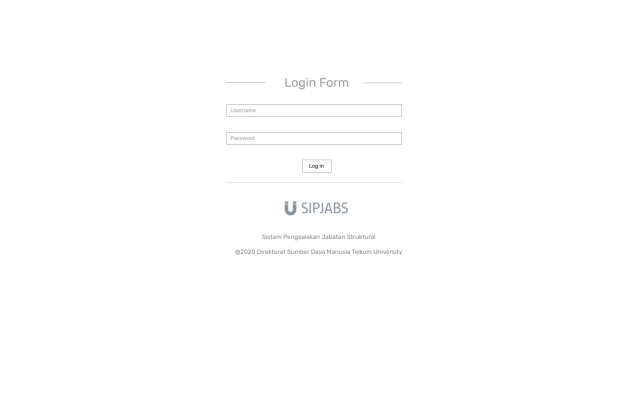
\includegraphics[width=0.6\textwidth, height=60mm]{pics/admin/login.jpg}} 
		& Halaman login merupakan tampilan awal apabila admin membuka aplikasi SiPJabS , admin dapat menginputkan username dan password untuk melakukan login. \\
	
		\hline
		
		2. & \raisebox{-\totalheight}{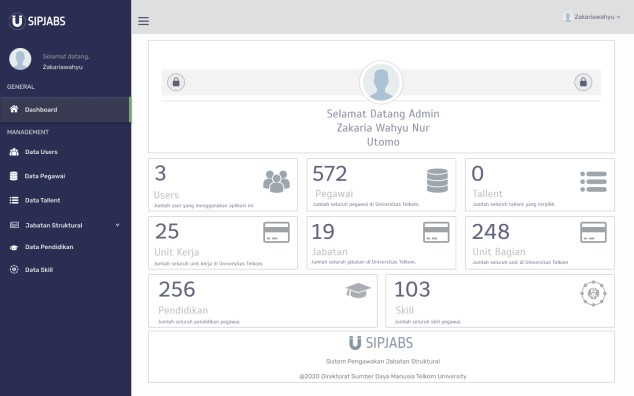
\includegraphics[width=0.6\textwidth, height=60mm]{pics/admin/dashboard.jpg}} 
		& Didalam dashboard admin terdapat jumlah users dari aplikasi SiPJabS, jumlah pegawai di Universitas Telkom, tallent yang sudah dipilih, unit kerja, jabatan, unit bagian, pendidikan dan skill yang dimiliki para pegawai  Universitas Telkom. \\
		\hline

	\end{tabular}
\end{table}


\begin{table}
	\caption{Tabel Perancangan Antar Muka Admin (1)}
	\centering
	\begin{tabular}{ | c | c | p{35mm} |}
		\hline 
		\textbf{No} & \textbf{Gambar} &  \textbf{Keterangan} \\ 
		\hline
		
		3. & \raisebox{-\totalheight}{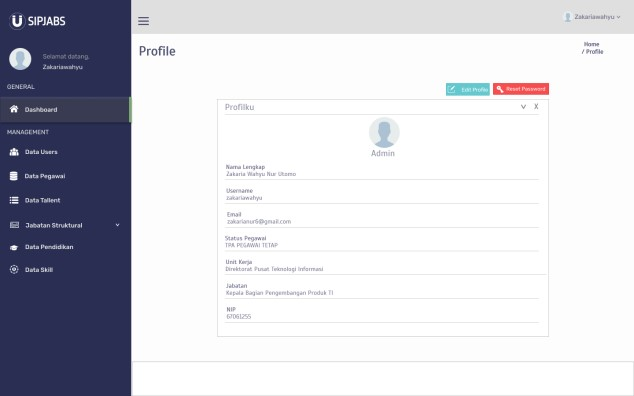
\includegraphics[width=0.6\textwidth, height=60mm]{pics/admin/profile.jpg}} 
		& Halaman profile admin akan menampilkan data profile dari admin tersebut. Kemudian admin juga dapat mengedit profile dan mereset password.  \\
		
		\hline
		
		4. & \raisebox{-\totalheight}{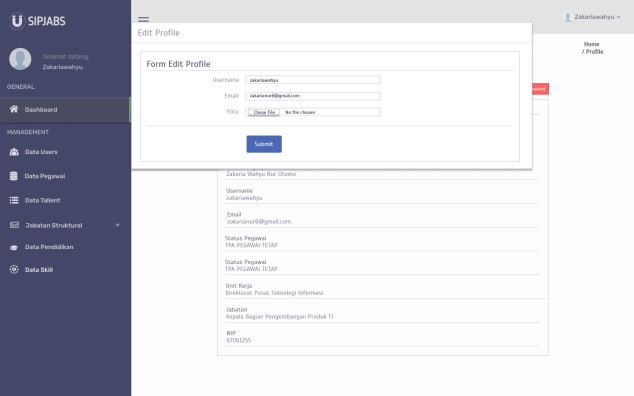
\includegraphics[width=0.6\textwidth, height=60mm]{pics/admin/editprofile.jpg}} 
		& Admin dapat mengubah username, menginputkan email, dan menambahkan foto profile.  \\
		
		\hline
		
		5. & \raisebox{-\totalheight}{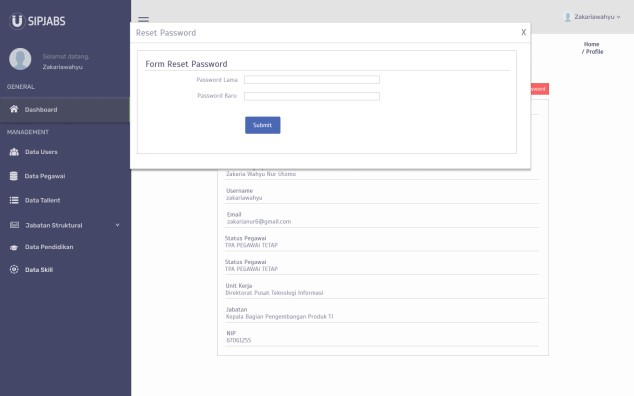
\includegraphics[width=0.6\textwidth, height=60mm]{pics/admin/resetpassword.jpg}} 
		& Admin harus menginputkan password yang lama serta yang baru, setelah itu admin dapat menyimpan. \\
		
		\hline
		
	\end{tabular}
\end{table}

\begin{table}
	\caption{Tabel Perancangan Antar Muka Admin (2)}
	\centering
	\begin{tabular}{ | c | c | p{35mm} |}
		\hline 
		\textbf{No} & \textbf{Gambar} &  \textbf{Keterangan} \\ 
		\hline
		
		
		
		6. & \raisebox{-\totalheight}{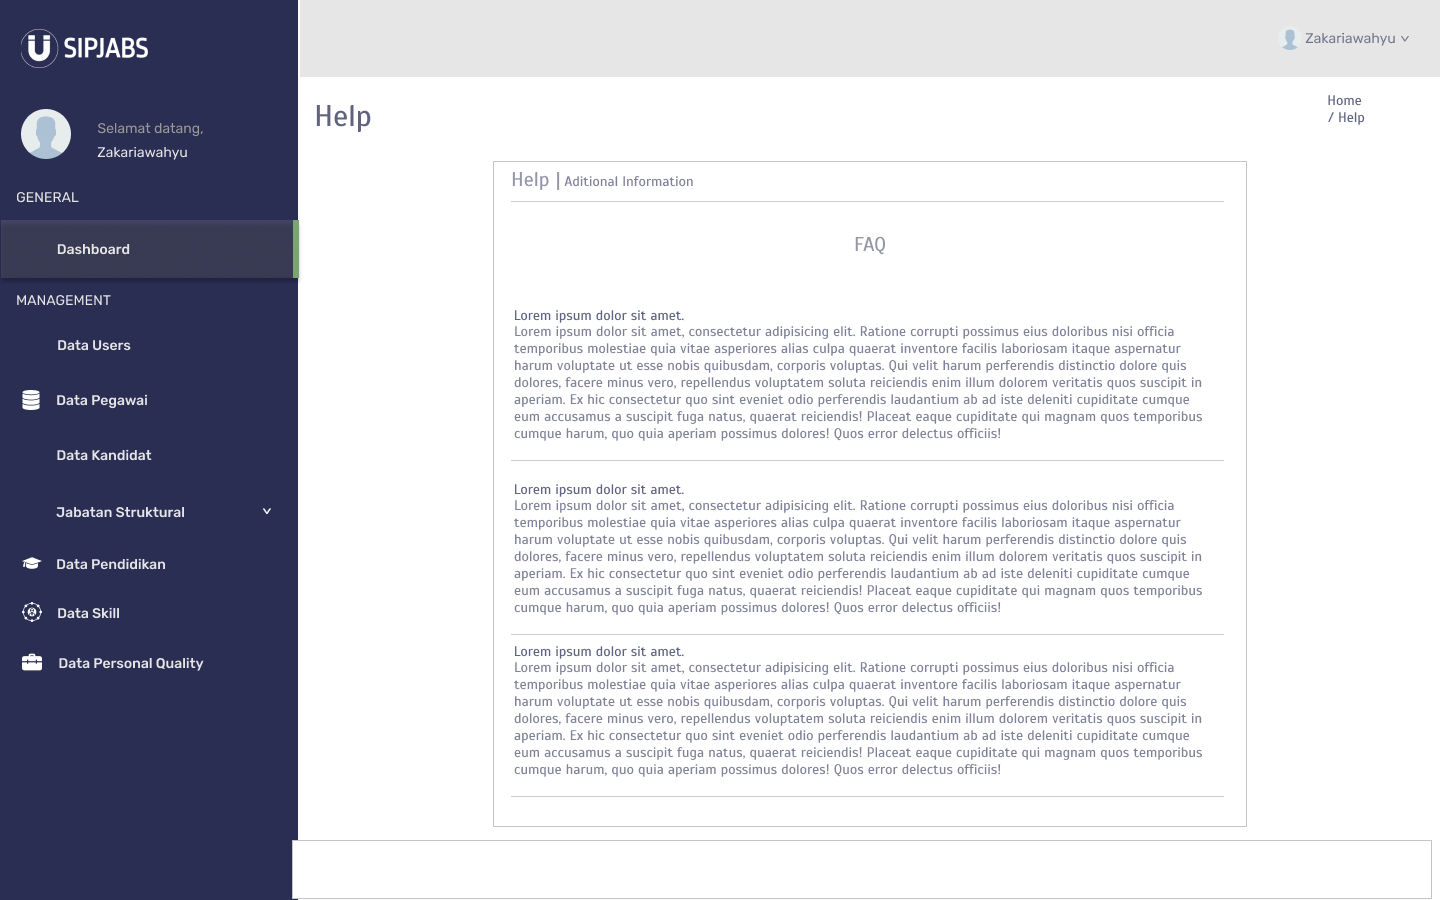
\includegraphics[width=0.6\textwidth, height=60mm]{pics/admin/help.png}} 
		& Halaman help berisi infomasi tentang aplikasi. \\
		
		\hline
		
		7. & \raisebox{-\totalheight}{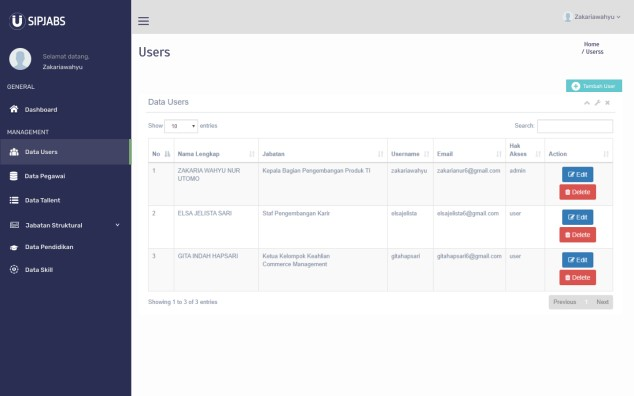
\includegraphics[width=0.6\textwidth, height=60mm]{pics/admin/datausers.jpg}} 
		& Halaman data user akan menampilkan nama-nama yang dapat mengakses aplikasi SiPJabS sebagai admin dan user. \\
		
		\hline
		
		8. & \raisebox{-\totalheight}{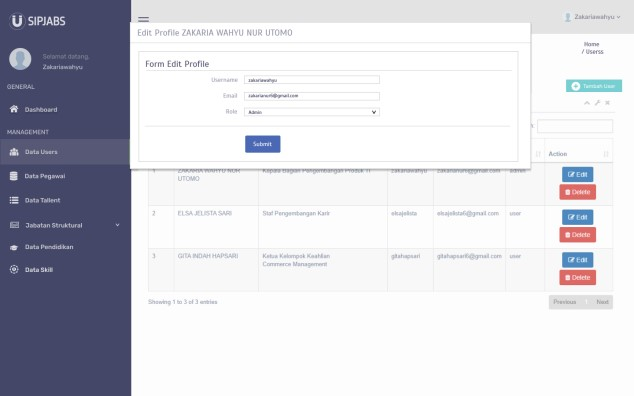
\includegraphics[width=0.6\textwidth, height=60mm]{pics/admin/editdatausers.jpg}} 
		& Pada halaman ini admin dapat mengedit username, email, dan role sebagai admin atau user. \\
		
		\hline
		
	\end{tabular}
\end{table}

\begin{table}
	\caption{Tabel Perancangan Antar Muka Admin (3)}
	\centering
	\begin{tabular}{ | c | c | p{35mm} |}
		\hline 
		\textbf{No} & \textbf{Gambar} &  \textbf{Keterangan} \\ 
		\hline
		
	
		
		9. & \raisebox{-\totalheight}{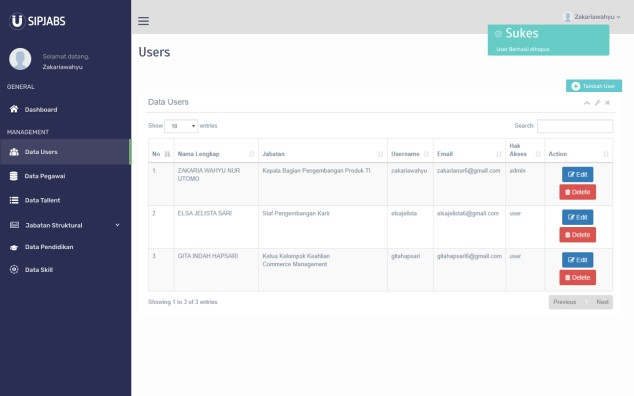
\includegraphics[width=0.6\textwidth, height=60mm]{pics/admin/hapususers.jpg}} 
		&Admin dapat menghapus data user apabila user tersebut sudah tidak bekerja pada bidangnya atau digantikan. \\
		
		\hline
		
		10. & \raisebox{-\totalheight}{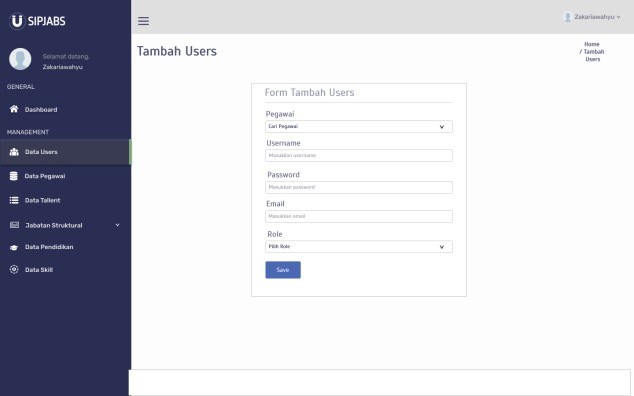
\includegraphics[width=0.6\textwidth, height=60mm]{pics/admin/tambahusers.jpg}} 
		& Admin dapat menambahkan user dengan mengisi form tambah user dan menyimpannya.. \\
		
		\hline
		
		11. & \raisebox{-\totalheight}{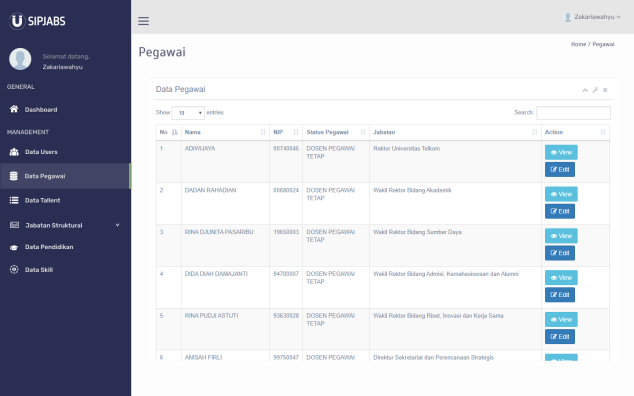
\includegraphics[width=0.6\textwidth, height=60mm]{pics/admin/datapegawai.png}} 
		& Admin dapat melihat daftar data pegawai yang ada di Universitas Telkom secara detail. \\
		
		\hline
		
	\end{tabular}
\end{table}

\begin{table}
	\caption{Tabel Perancangan Antar Muka Admin (4)}
	\centering
	\begin{tabular}{ | c | c | p{35mm} |}
		\hline 
		\textbf{No} & \textbf{Gambar} &  \textbf{Keterangan} \\ 
		\hline
		
		
		
		12. & \raisebox{-\totalheight}{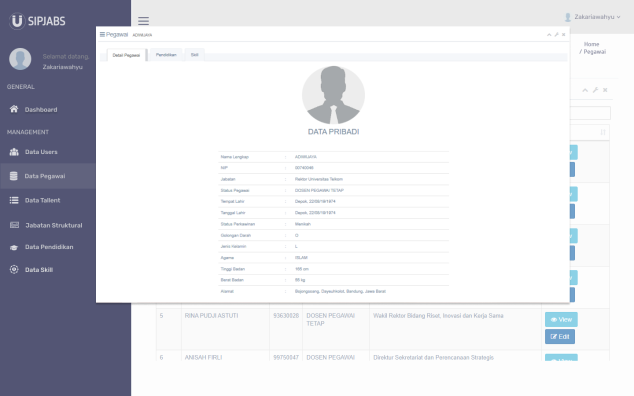
\includegraphics[width=0.6\textwidth, height=60mm]{pics/admin/viewdetailpegawai.png}} 
		&Halaman ini akan menampilkan data pribadi dari pegawai.  \\
		
		\hline
		
		13. & \raisebox{-\totalheight}{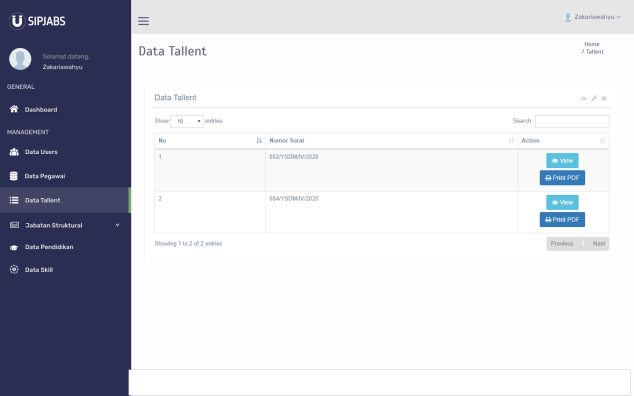
\includegraphics[width=0.6\textwidth, height=60mm]{pics/admin/datatallent.png}} 
		& Halaman ini akan menampilkan data tallent yang sudah di pilih oleh user sesuai dengan job description untuk menggantikan atau mengisi posisi yang kosong. \\
		
		\hline
		
		14. & \raisebox{-\totalheight}{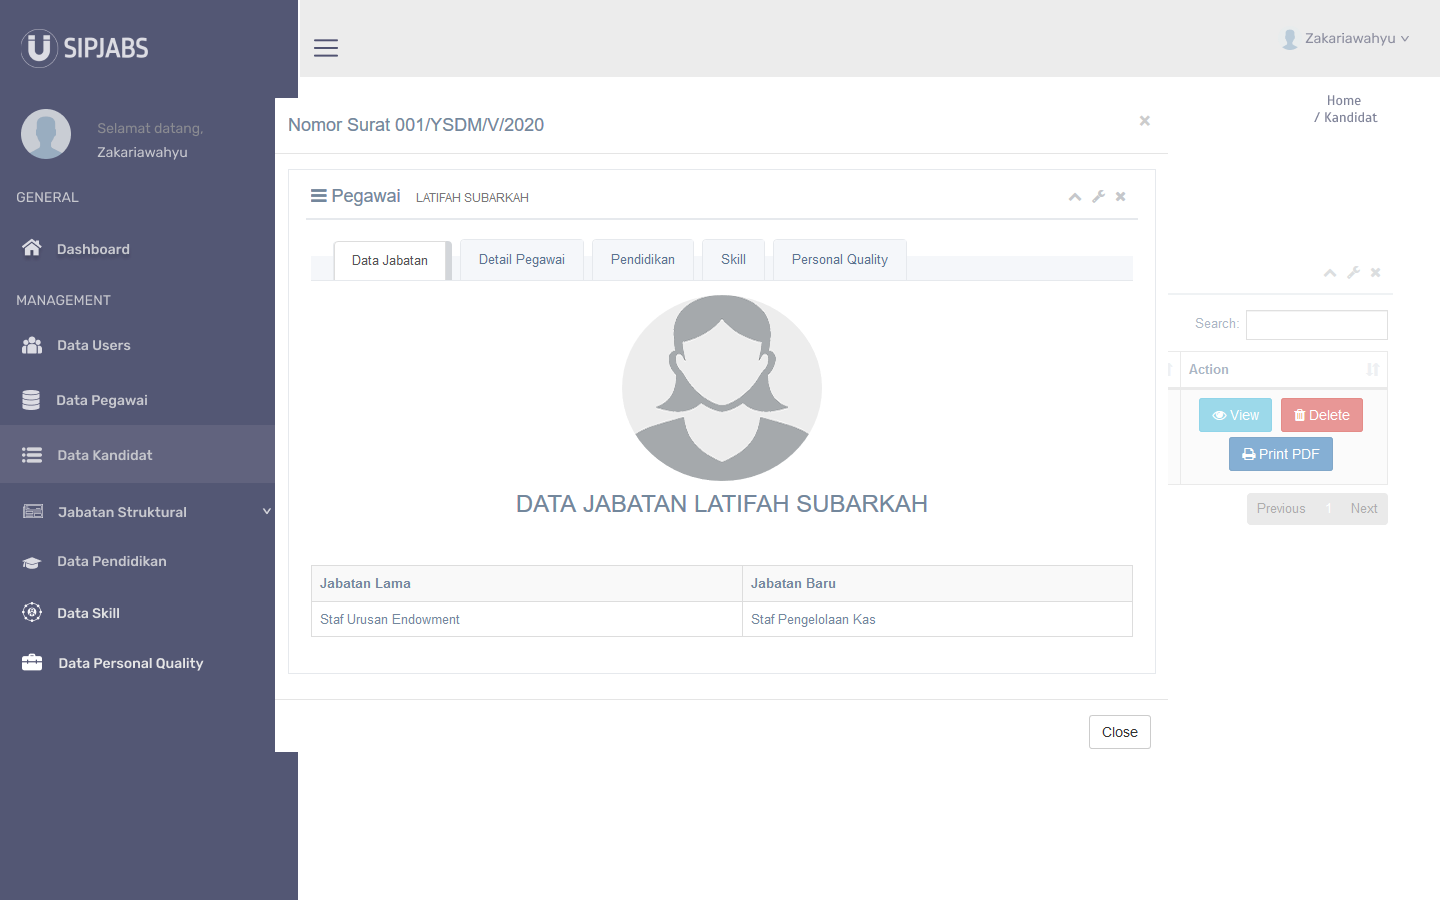
\includegraphics[width=0.6\textwidth, height=60mm]{pics/admin/viewdetailtallent.png}} 
		& Admin dapat melihat data detail tallent yang sudah dipilih. \\
		
		\hline
		
	\end{tabular}
\end{table}

\begin{table}
	\caption{Tabel Perancangan Antar Muka Admin (5)}
	\centering
	\begin{tabular}{ | c | c | p{35mm} |}
		\hline 
		\textbf{No} & \textbf{Gambar} &  \textbf{Keterangan} \\ 
		\hline
		
		
		
		15. & \raisebox{-\totalheight}{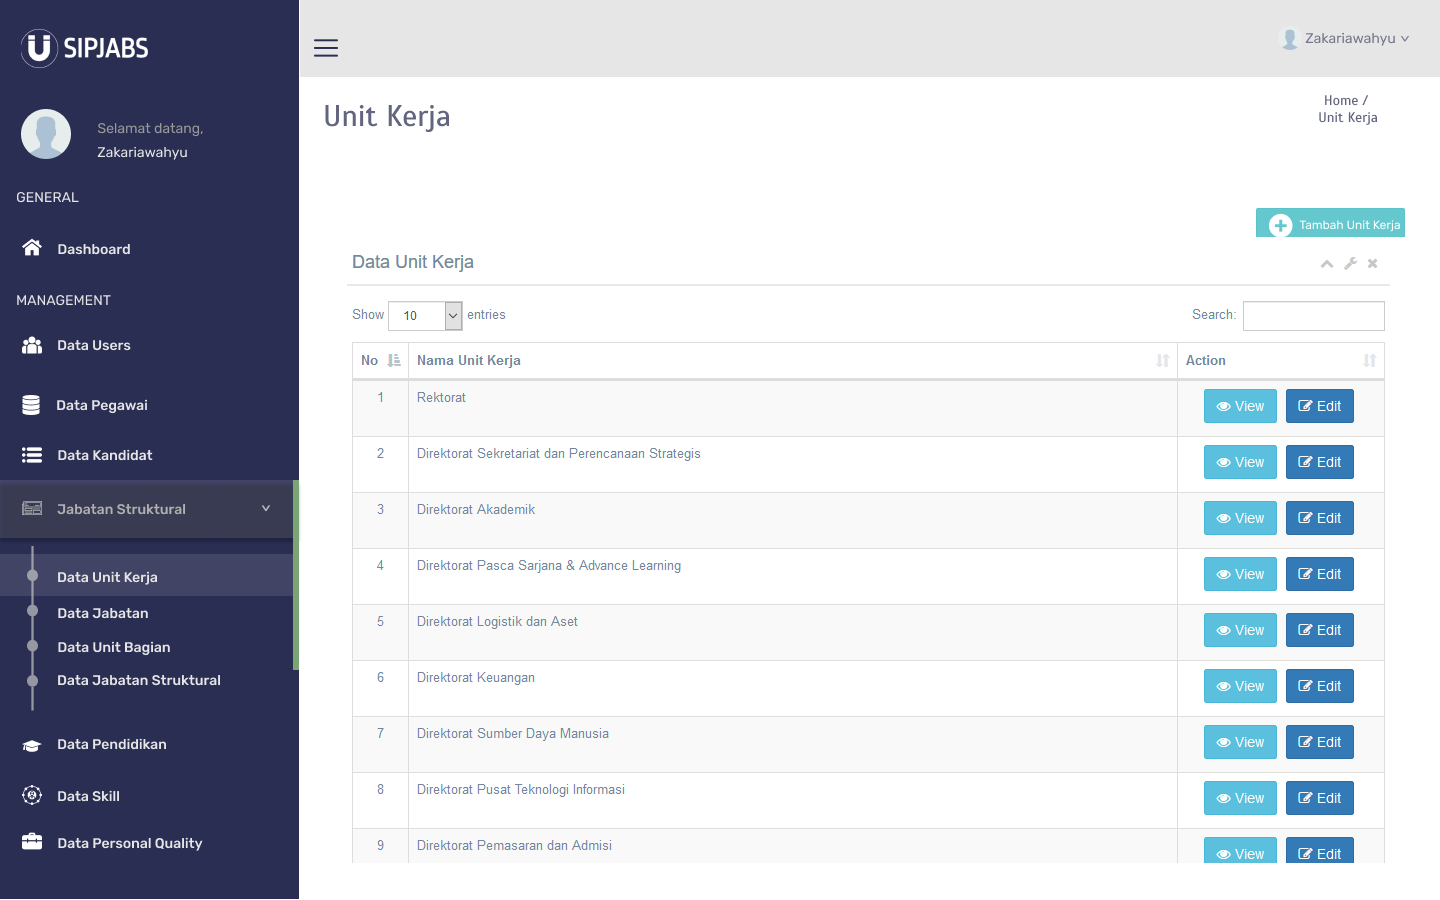
\includegraphics[width=0.6\textwidth, height=60mm]{pics/admin/dataunitkerja.png}} 
		&Halaman ini akan menunjukkan semua unit kerja dimulai dari rektorat hingga fakultas yang ada di Universitas Telkom. \\
		
		\hline
		
		16. & \raisebox{-\totalheight}{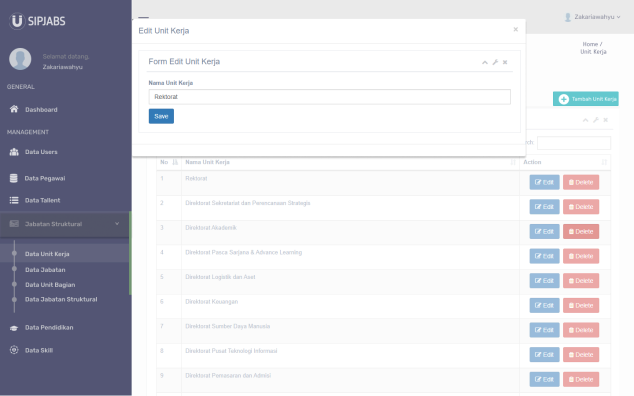
\includegraphics[width=0.6\textwidth, height=60mm]{pics/admin/editunitkerja.png}} 
		& Admin dapat mengedit form unit kerja apabila terdapat kebijakan baru. \\
		
		\hline
		
		17. & \raisebox{-\totalheight}{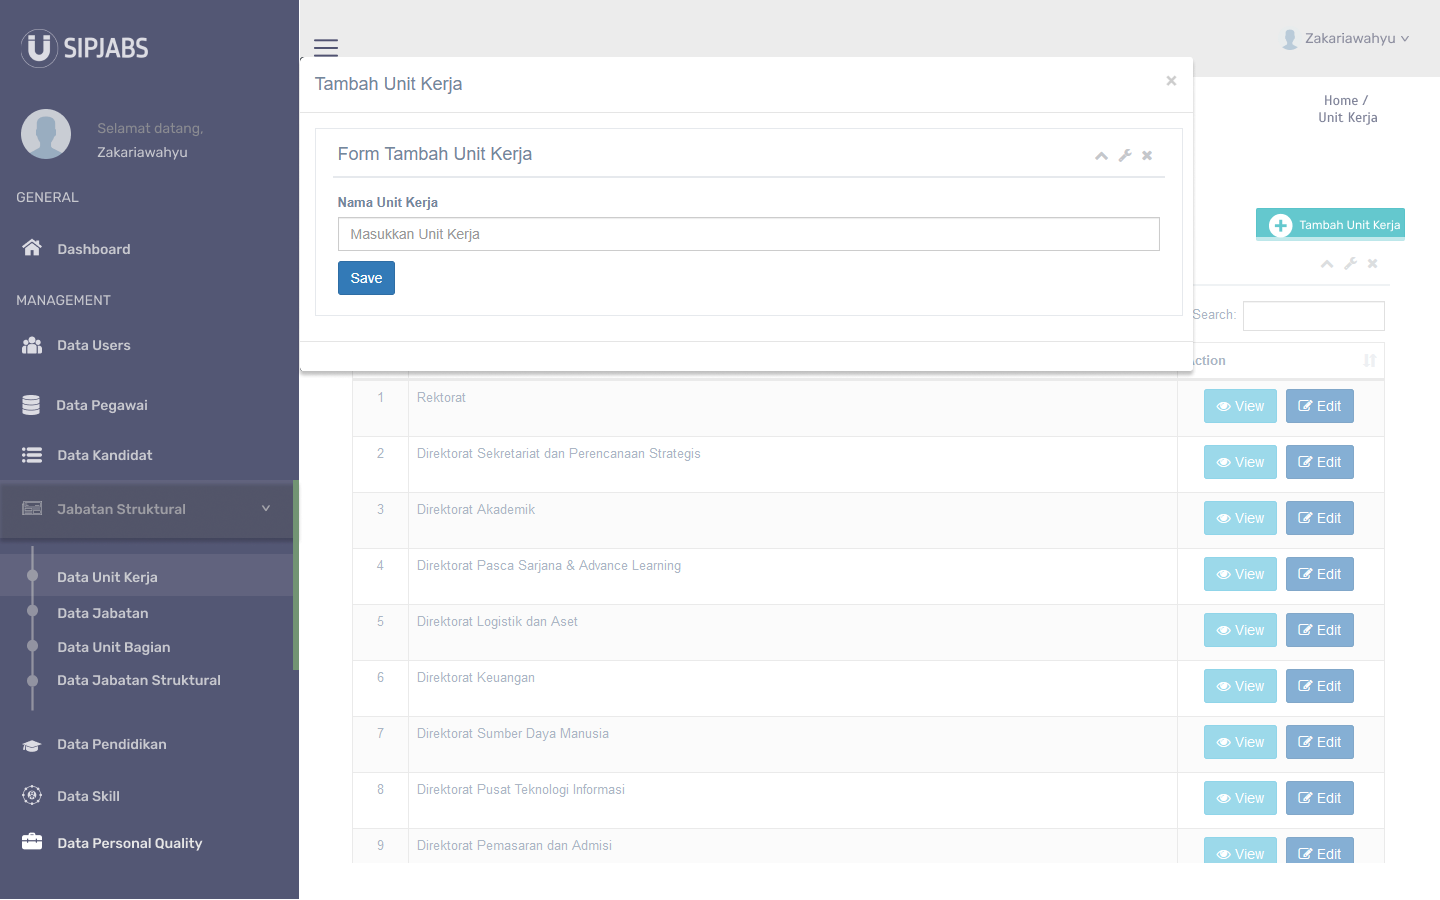
\includegraphics[width=0.6\textwidth, height=60mm]{pics/admin/tambahunitkerja.png}} 
		& Admin dapat menambahkan data unit kerja dengan mengisi form tersebut, namun harus sesuai dengan kebijakan yang telah ditetapkan. \\
		
		\hline
		
	\end{tabular}
\end{table}

\begin{table}
	\caption{Tabel Perancangan Antar Muka Admin (6)}
	\centering
	\begin{tabular}{ | c | c | p{35mm} |}
		\hline 
		\textbf{No} & \textbf{Gambar} &  \textbf{Keterangan} \\ 
		\hline
		
	
		
		18. & \raisebox{-\totalheight}{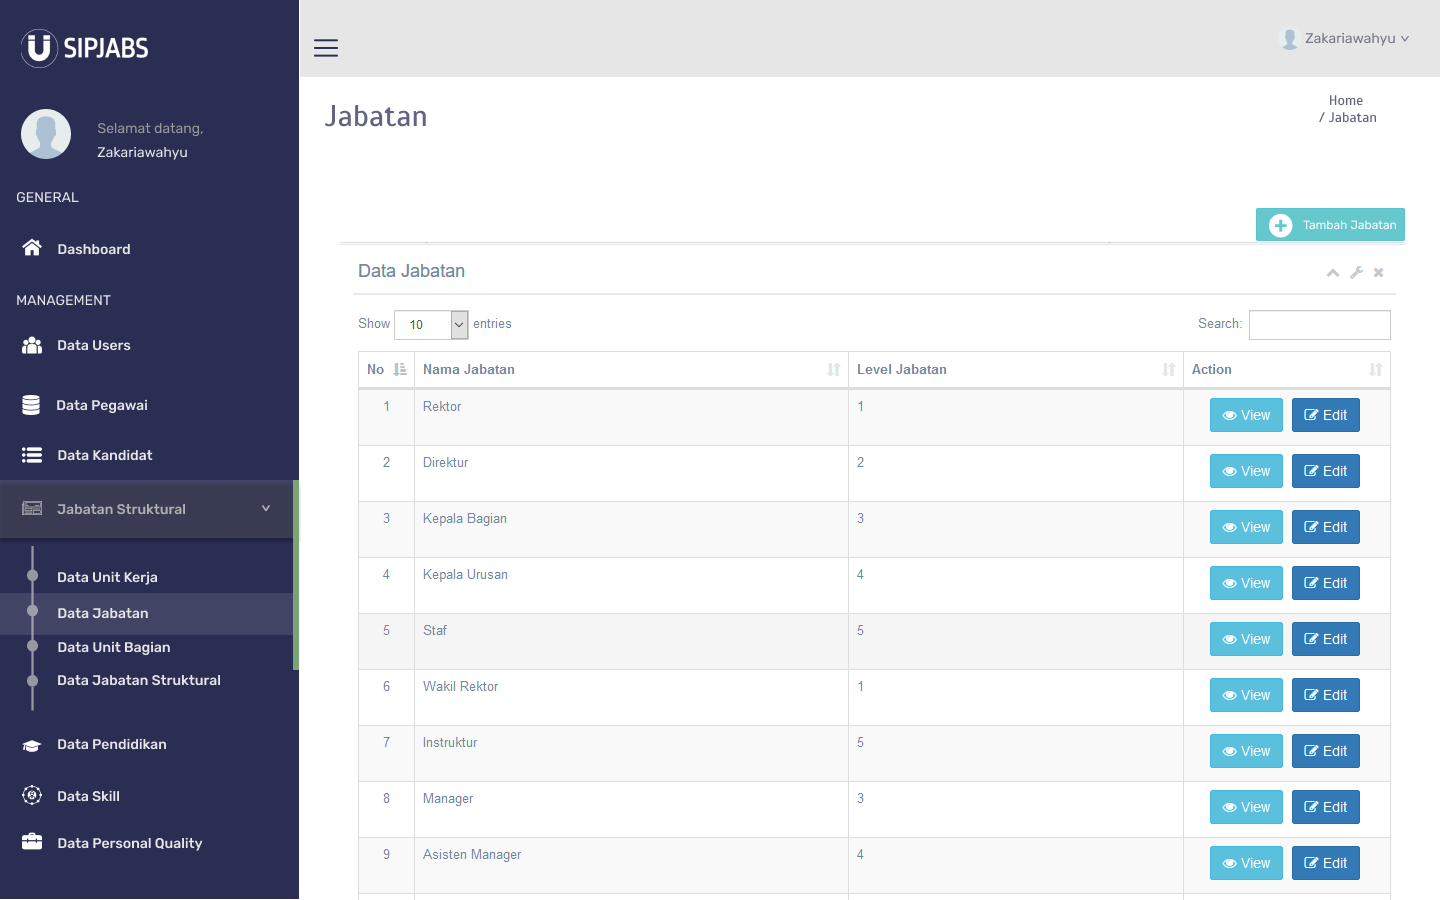
\includegraphics[width=0.6\textwidth, height=60mm]{pics/admin/datajabatan.png}} 
		&Halaman ini akan menampilkan data jabatan yang berada di Universitas Telkom \\
		
		\hline
		
		19. & \raisebox{-\totalheight}{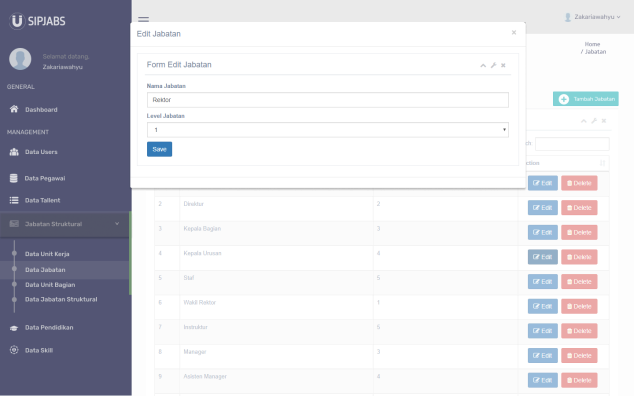
\includegraphics[width=0.6\textwidth, height=60mm]{pics/admin/editjabatan.png}} 
		& Admin dapat mengedit data jabatan sesuai dengan nama jabatan yang sudah ditetapkan. \\
		
		\hline
		
		20. & \raisebox{-\totalheight}{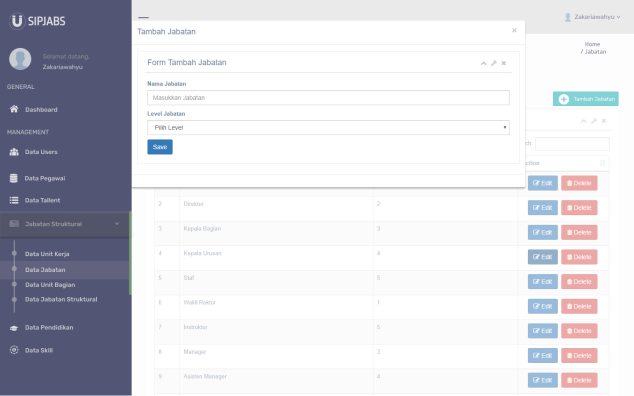
\includegraphics[width=0.6\textwidth, height=60mm]{pics/admin/tambahjabatan.png}} 
		& Admin harus melengkapi form tersebut untuk dapat menambahkan data jabatan yang baru. \\
		
		\hline
		
	\end{tabular}
\end{table}

\begin{table}
	\caption{Tabel Perancangan Antar Muka Admin (7)}
	\centering
	\begin{tabular}{ | c | c | p{35mm} |}
		\hline 
		\textbf{No} & \textbf{Gambar} &  \textbf{Keterangan} \\ 
		\hline
		
		
		
		21. & \raisebox{-\totalheight}{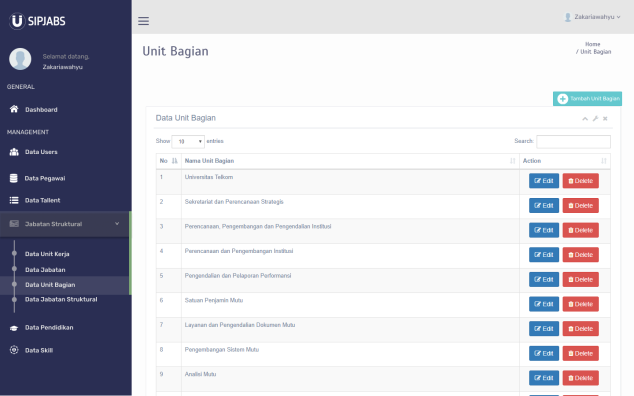
\includegraphics[width=0.6\textwidth, height=60mm]{pics/admin/dataunitbagian.png}} 
		&Halaman ini akan menampilkan satuan kerja yang terdapat di Universitas Telkom.  \\
		
		\hline
		
		22. & \raisebox{-\totalheight}{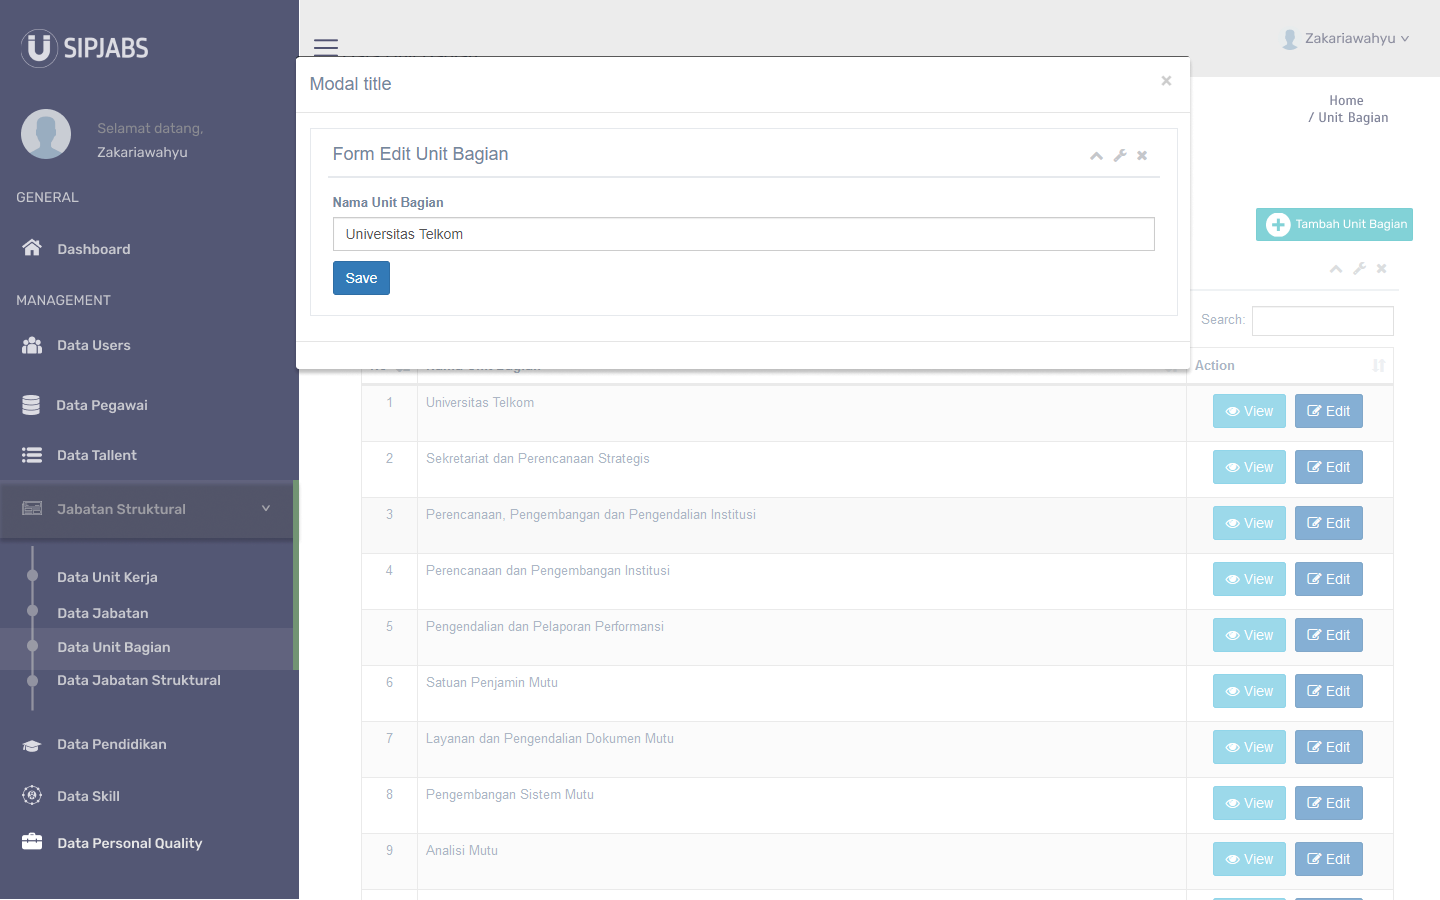
\includegraphics[width=0.6\textwidth, height=60mm]{pics/admin/editunitbagian.png}} 
		& Admin dapat mengedit data unit bagian apabila ada perubahan yang sudah ditetapkan.\\
		
		\hline
		
		23. & \raisebox{-\totalheight}{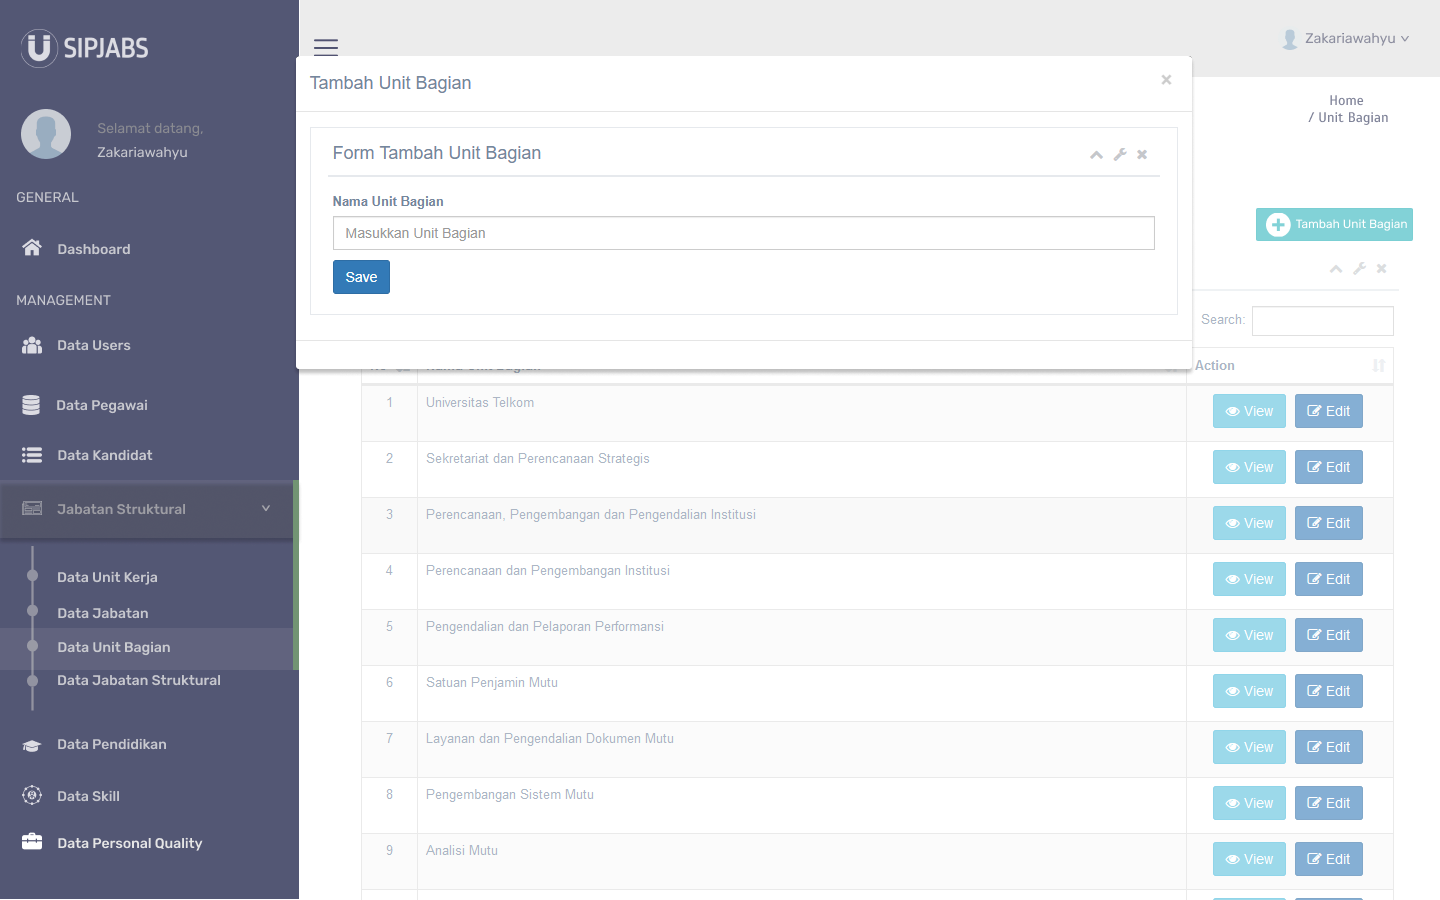
\includegraphics[width=0.6\textwidth, height=60mm]{pics/admin/tambahunitbagian.png}} 
		& Admin harus menginputkan  nama unit bagian  tersebut untuk dapat menambahkan data data unit bagian yang baru. \\
		
		\hline
		
	\end{tabular}
\end{table}

\begin{table}
	\caption{Tabel Perancangan Antar Muka Admin (8)}
	\centering
	\begin{tabular}{ | c | c | p{35mm} |}
		\hline 
		\textbf{No} & \textbf{Gambar} &  \textbf{Keterangan} \\ 
		\hline
		
		
		
		24. & \raisebox{-\totalheight}{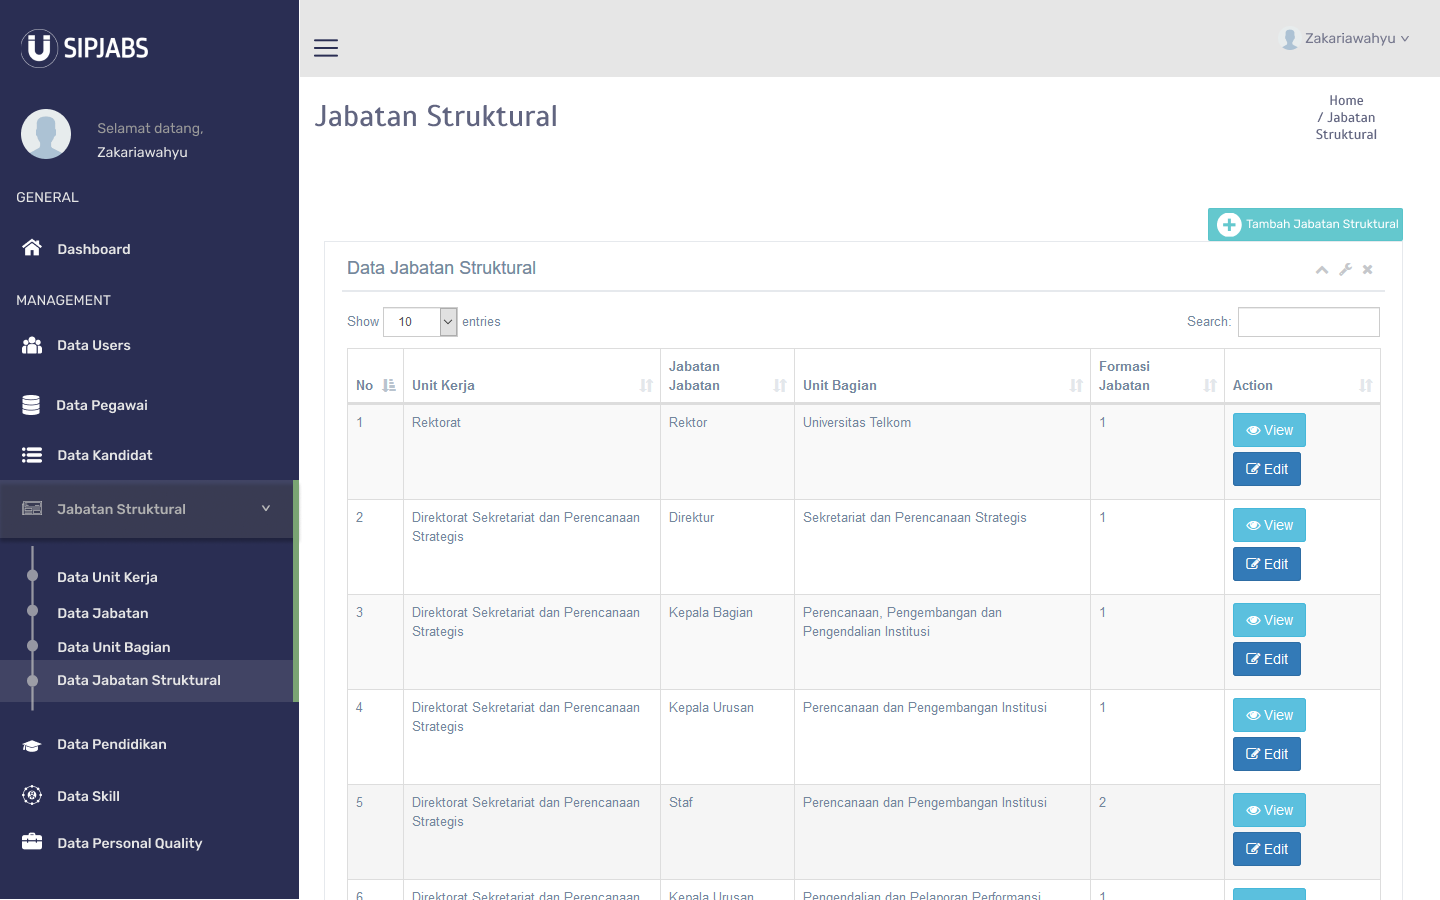
\includegraphics[width=0.6\textwidth, height=60mm]{pics/admin/datajabstruk.png}} 
		&Halaman ini menampilkan jabatan yang secara tegas ada di Universitas Telkom.  \\
		
		\hline
		
		25. & \raisebox{-\totalheight}{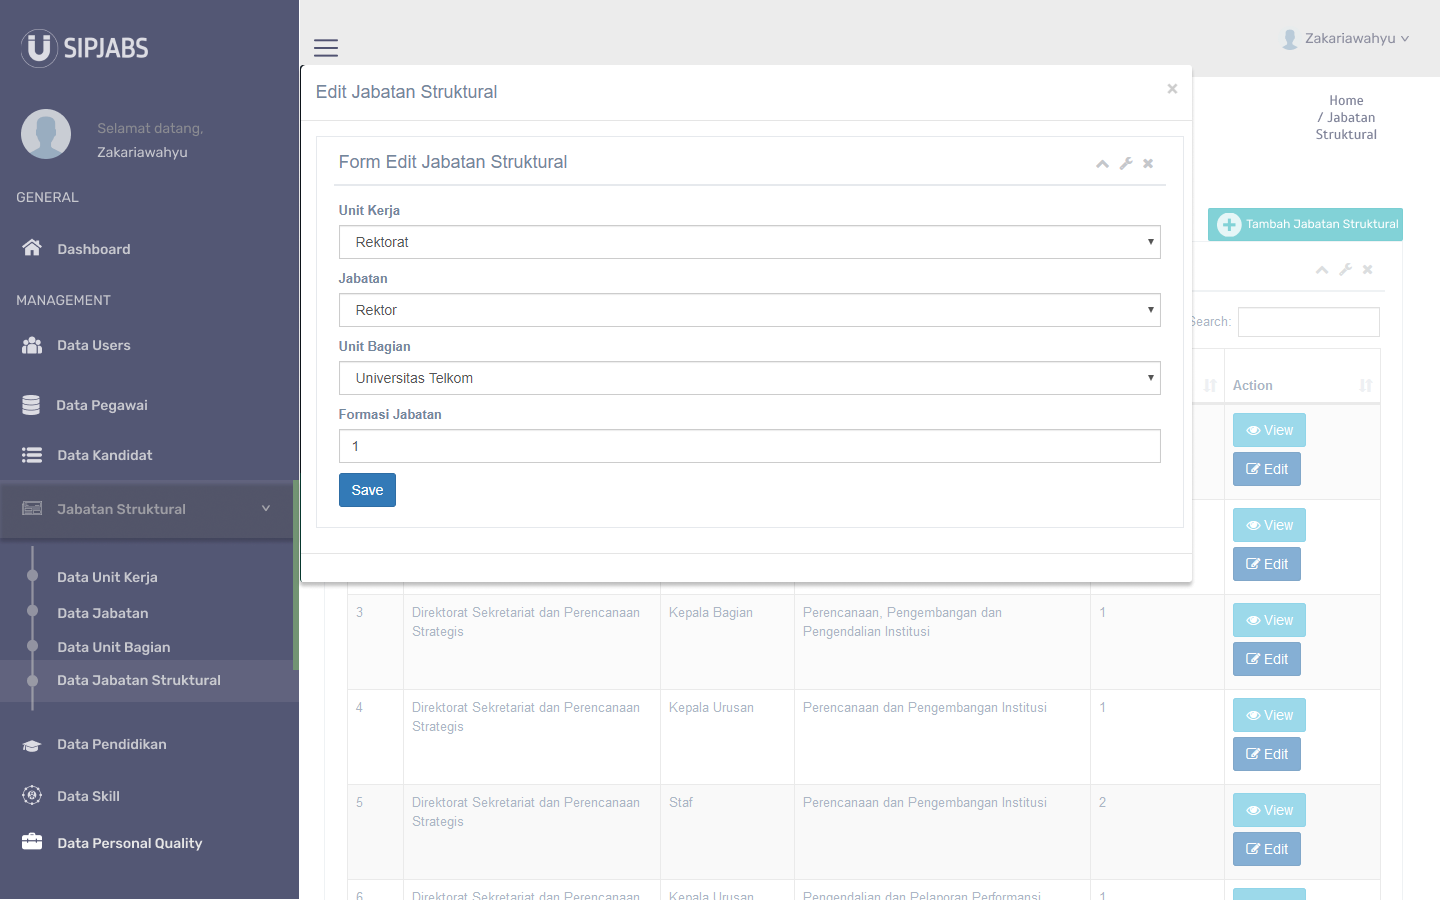
\includegraphics[width=0.6\textwidth, height=60mm]{pics/admin/editjabstruk.png}} 
		& Admin dapat mengedit data dan harus mengisi form sesuai dengan ketetapan.\\
		
		\hline
		
		26. & \raisebox{-\totalheight}{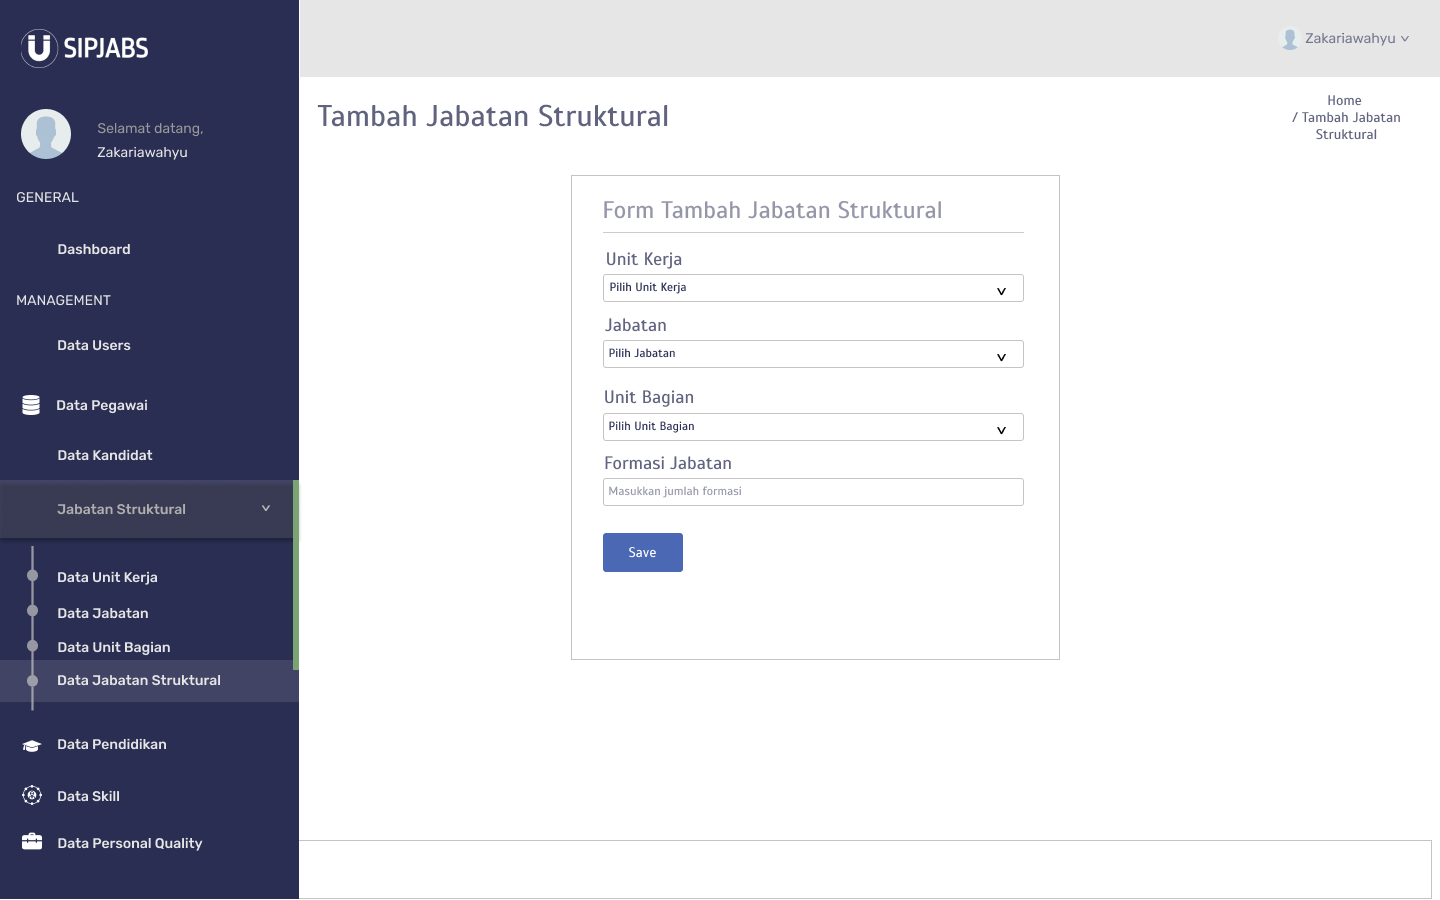
\includegraphics[width=0.6\textwidth, height=60mm]{pics/admin/tambahjabstruk.png}} 
		& Admin harus melengkapi form untuk dapat menambahkan data jabatan struktural baru yang sudah ditetapkan. \\
		
		\hline
		
	\end{tabular}
\end{table}

\begin{table}
	\caption{Tabel Perancangan Antar Muka Admin (9)}
	\centering
	\begin{tabular}{ | c | c | p{35mm} |}
		\hline 
		\textbf{No} & \textbf{Gambar} &  \textbf{Keterangan} \\ 
		\hline
		
		
		
		27. & \raisebox{-\totalheight}{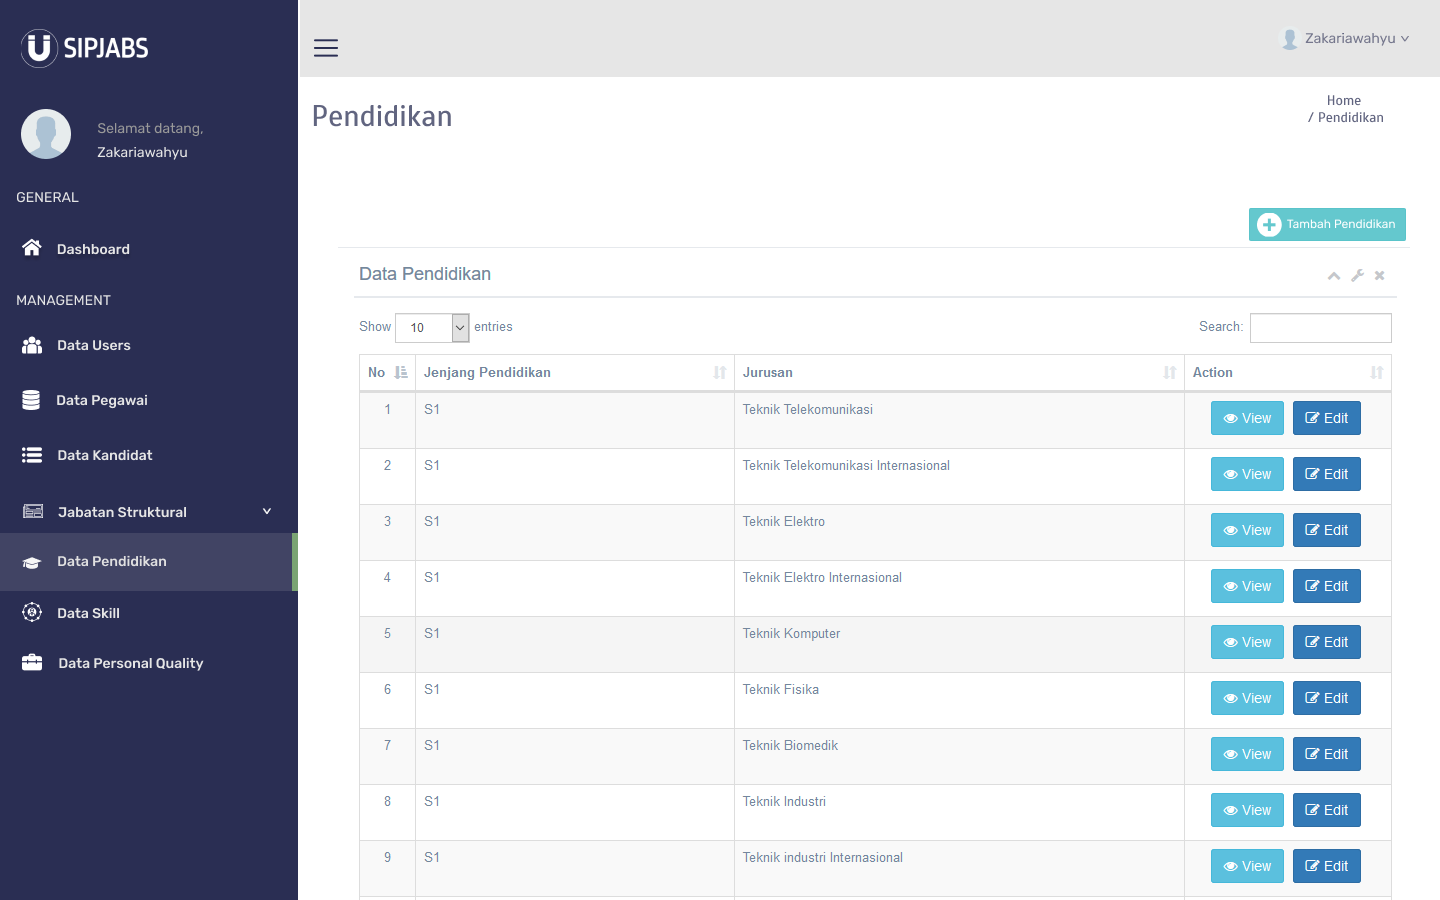
\includegraphics[width=0.6\textwidth, height=60mm]{pics/admin/datapendidikan.png}} 
		&Halaman ini akan menampilkan data pendidikan yang dimiliki pegawai Universitas Telkom.  \\
		
		\hline
		
		28. & \raisebox{-\totalheight}{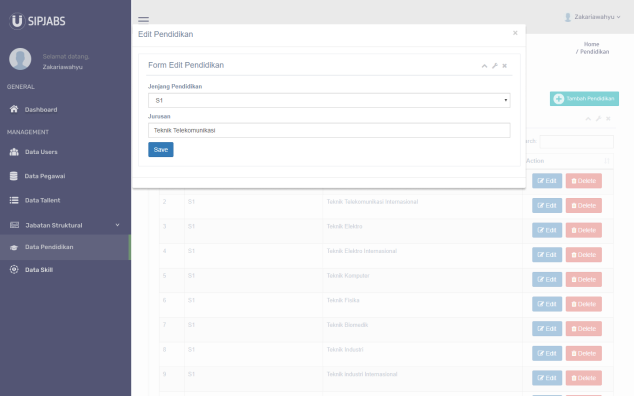
\includegraphics[width=0.6\textwidth, height=60mm]{pics/admin/editpendidikan.png}} 
		& Apabila ingin mengedit maka admin harus menginputkan jenjang pendidikan serta jurusan. \\
		
		\hline
		
		29. & \raisebox{-\totalheight}{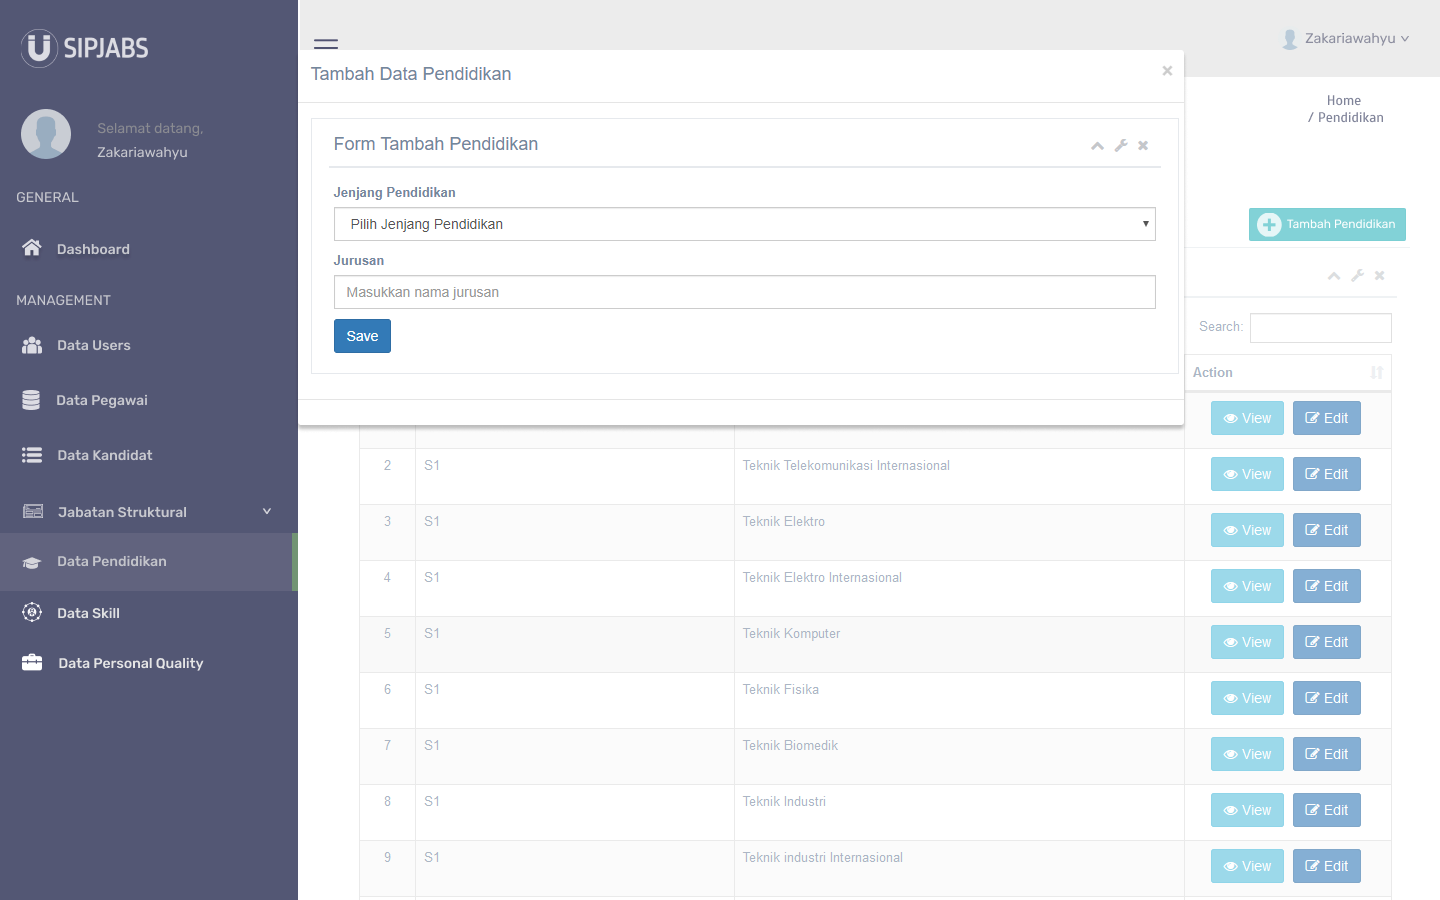
\includegraphics[width=0.6\textwidth, height=60mm]{pics/admin/tambahpendidikan.png}} 
		& Admin dapat menambahkan data pendidikan apabila belum ada data pendidikan yang dimiliki pegawai belum terinput. \\
		
		\hline
		
	\end{tabular}
\end{table}

\begin{table}
	\caption{Tabel Perancangan Antar Muka Admin (10)}
	\centering
	\begin{tabular}{ | c | c | p{35mm} |}
		\hline 
		\textbf{No} & \textbf{Gambar} &  \textbf{Keterangan} \\ 
		\hline
		
		
		
		30. & \raisebox{-\totalheight}{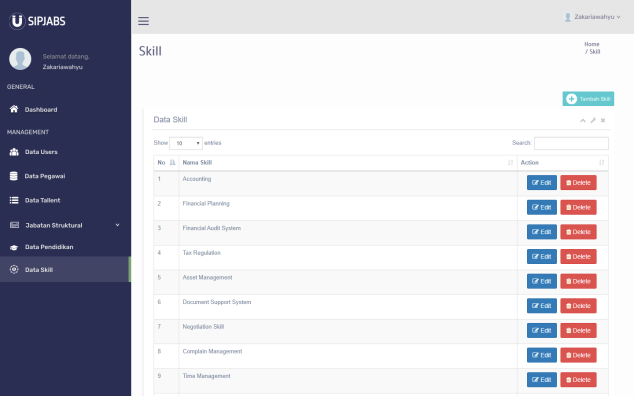
\includegraphics[width=0.6\textwidth, height=60mm]{pics/admin/dataskill.png}} 
		&Halaman ini akan menampilkan skill yang dimiliki pegawai Universitas Telkom untuk menunjang pekerjaan.  \\
		
		\hline
		
		31. & \raisebox{-\totalheight}{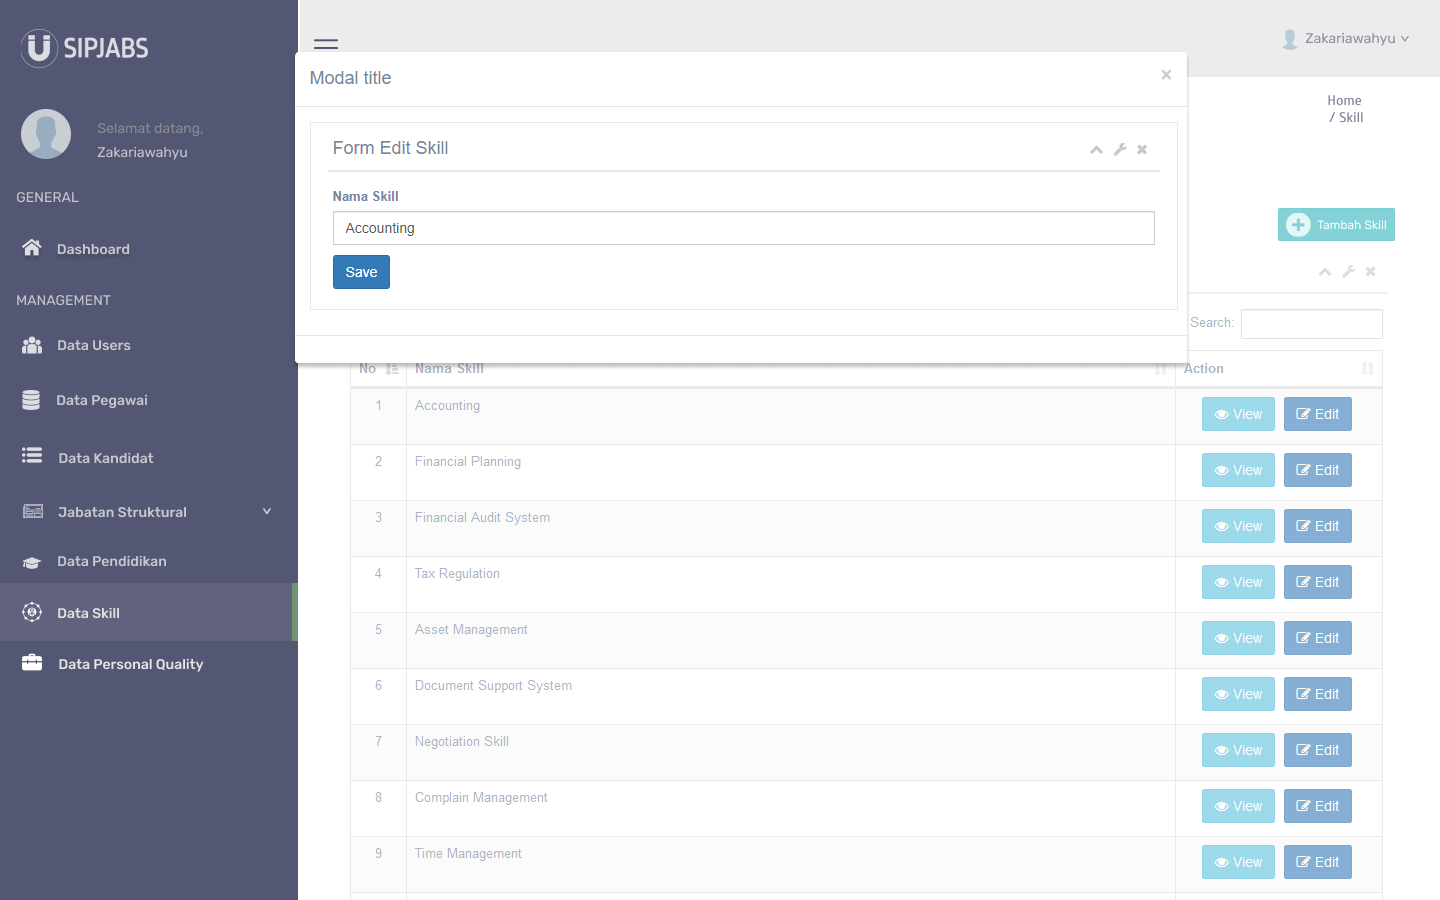
\includegraphics[width=0.6\textwidth, height=60mm]{pics/admin/editskill.png}} 
		& Admin dapat mengedit data skill. \\
		
		\hline
		
		32. & \raisebox{-\totalheight}{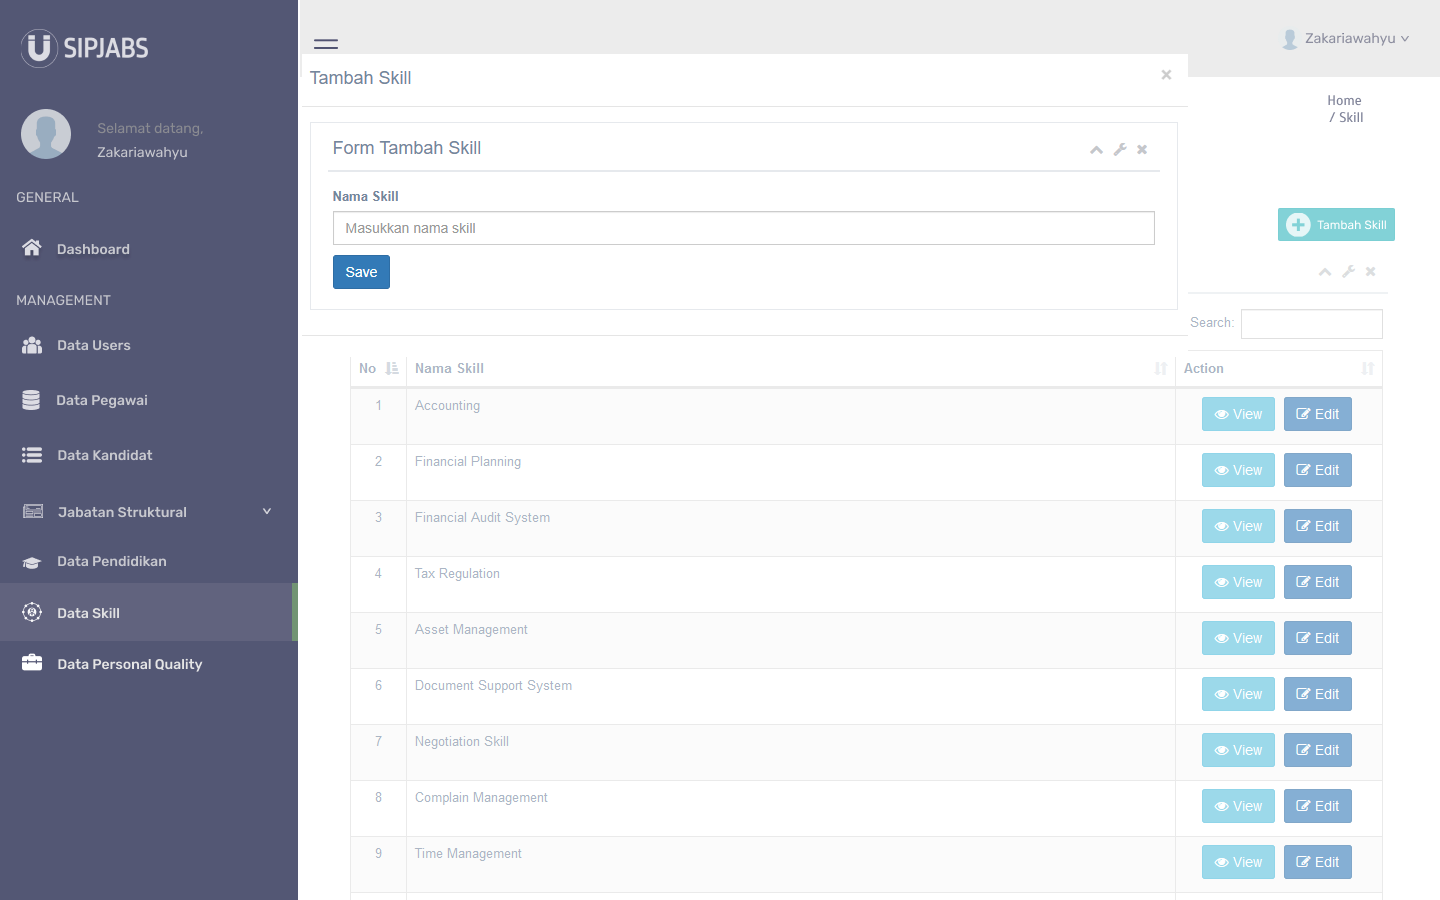
\includegraphics[width=0.6\textwidth, height=60mm]{pics/admin/tambahskill.png}} 
		& Admin dapat menambahkan data skill baru apabila terdapat data skill yang belum diinputkan.  \\
		
		\hline
		
	\end{tabular}
\end{table}

\subsubsection{Perancangan Antar Muka User}

\begin{table}
	\caption{Tabel Perancangan Antar Muka User}
	\centering
	\begin{tabular}{ | c | c | p{35mm} |}
		\hline 
		\textbf{No} & \textbf{Gambar} &  \textbf{Keterangan} \\ 
		\hline
		
		1. & \raisebox{-\totalheight}{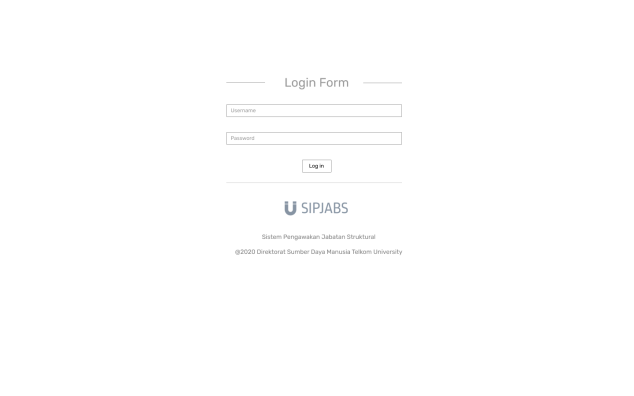
\includegraphics[width=0.6\textwidth, height=60mm]{pics/user/login.png}} 
		& Halaman login merupakan tampilan awal apabila user membuka aplikasi SiPJabS ,user dapat menginputkan username dan password untuk melakukan login.  \\
		
		\hline
		
		2. & \raisebox{-\totalheight}{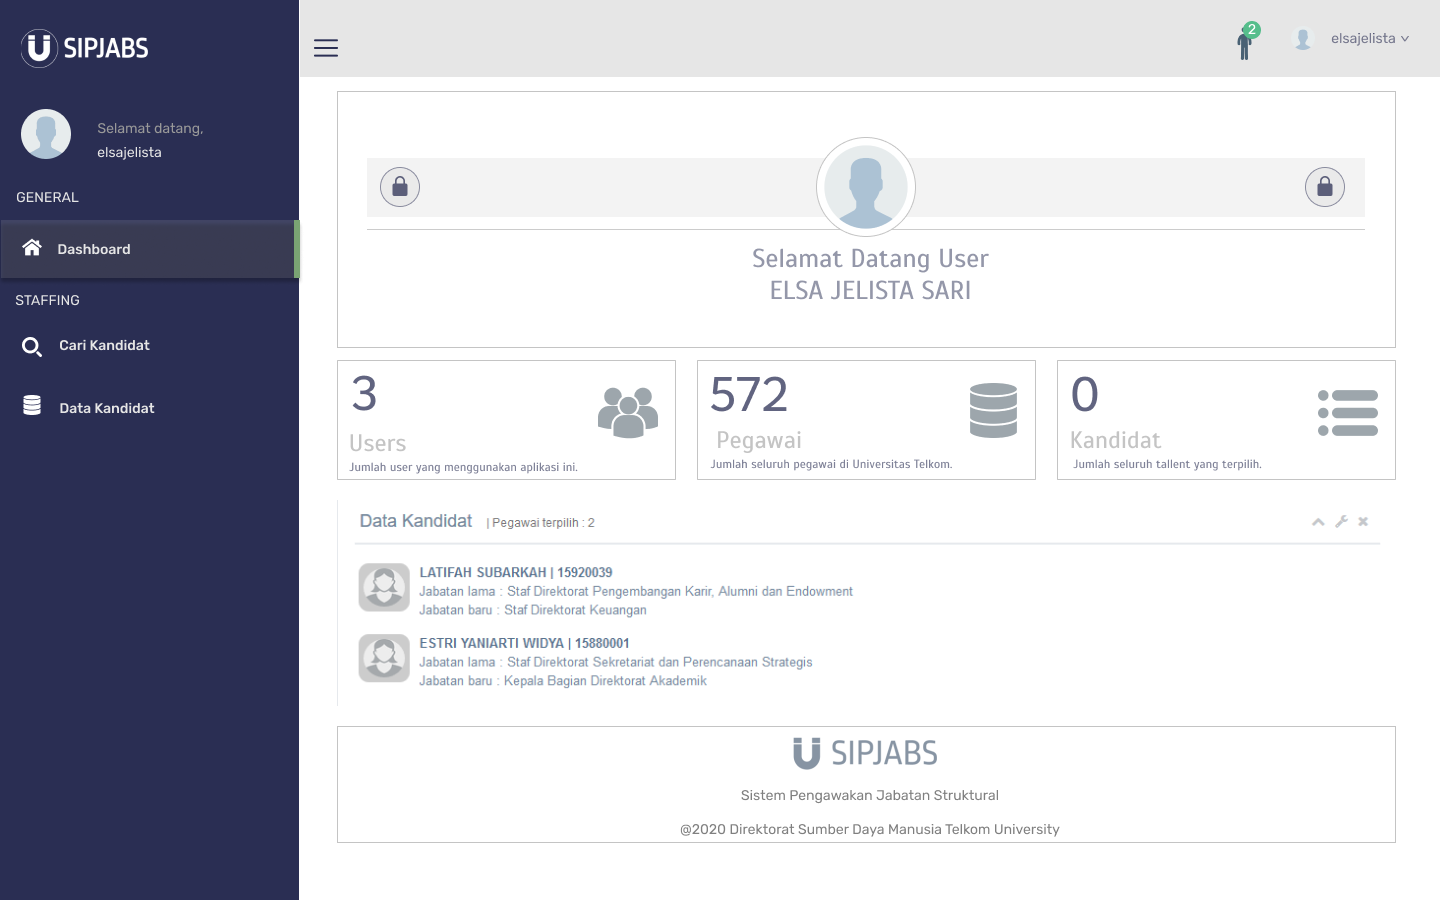
\includegraphics[width=0.6\textwidth, height=60mm]{pics/user/dashboard.png}} 
		& Halaman ini akan menampilkan jumlah user yang dapat mengakses aplikasi SiPJabS, jumlah pegawai yang ada di Universitas Telkom serta jumlah tallent yang sudah dipilih.  \\
		
		\hline
		
		3. & \raisebox{-\totalheight}{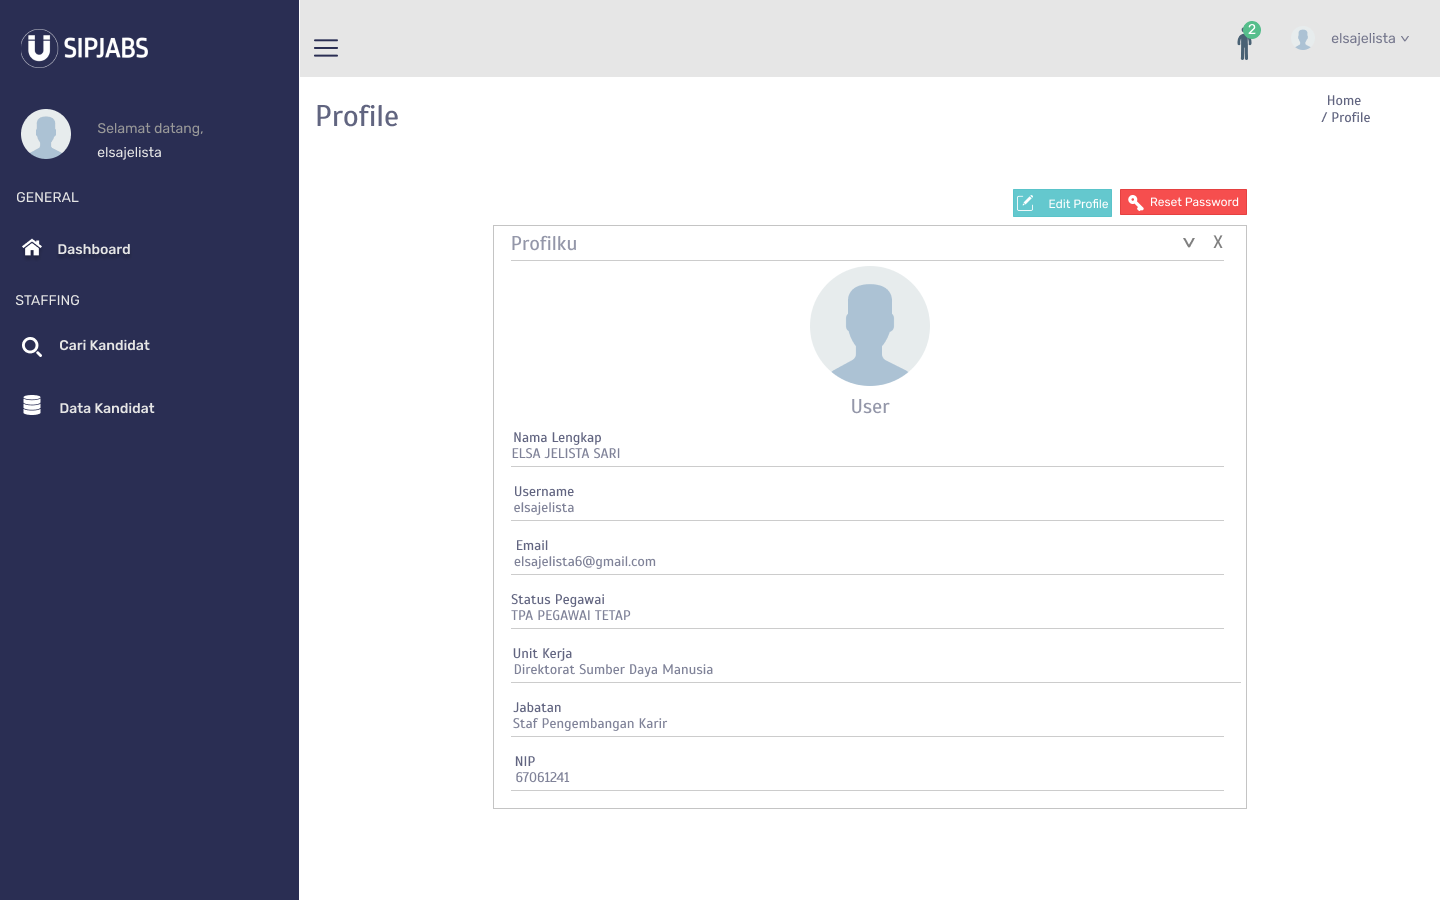
\includegraphics[width=0.6\textwidth, height=60mm]{pics/user/profile.png}} 
		& Halaman profile user akan menampilkan data nama lengkap, username, email, status pegawai, unit kerja, jabatan, serta NIP dari user tersebut. Kemudian user juga dapat mengedit profile dan mereset password.\\
		
		\hline
		
		
	\end{tabular}
\end{table}

\begin{table}
	\caption{Tabel Perancangan Antar Muka User (1)}
	\centering
	\begin{tabular}{ | c | c | p{35mm} |}
		\hline 
		\textbf{No} & \textbf{Gambar} &  \textbf{Keterangan} \\ 
		\hline
		
		4. & \raisebox{-\totalheight}{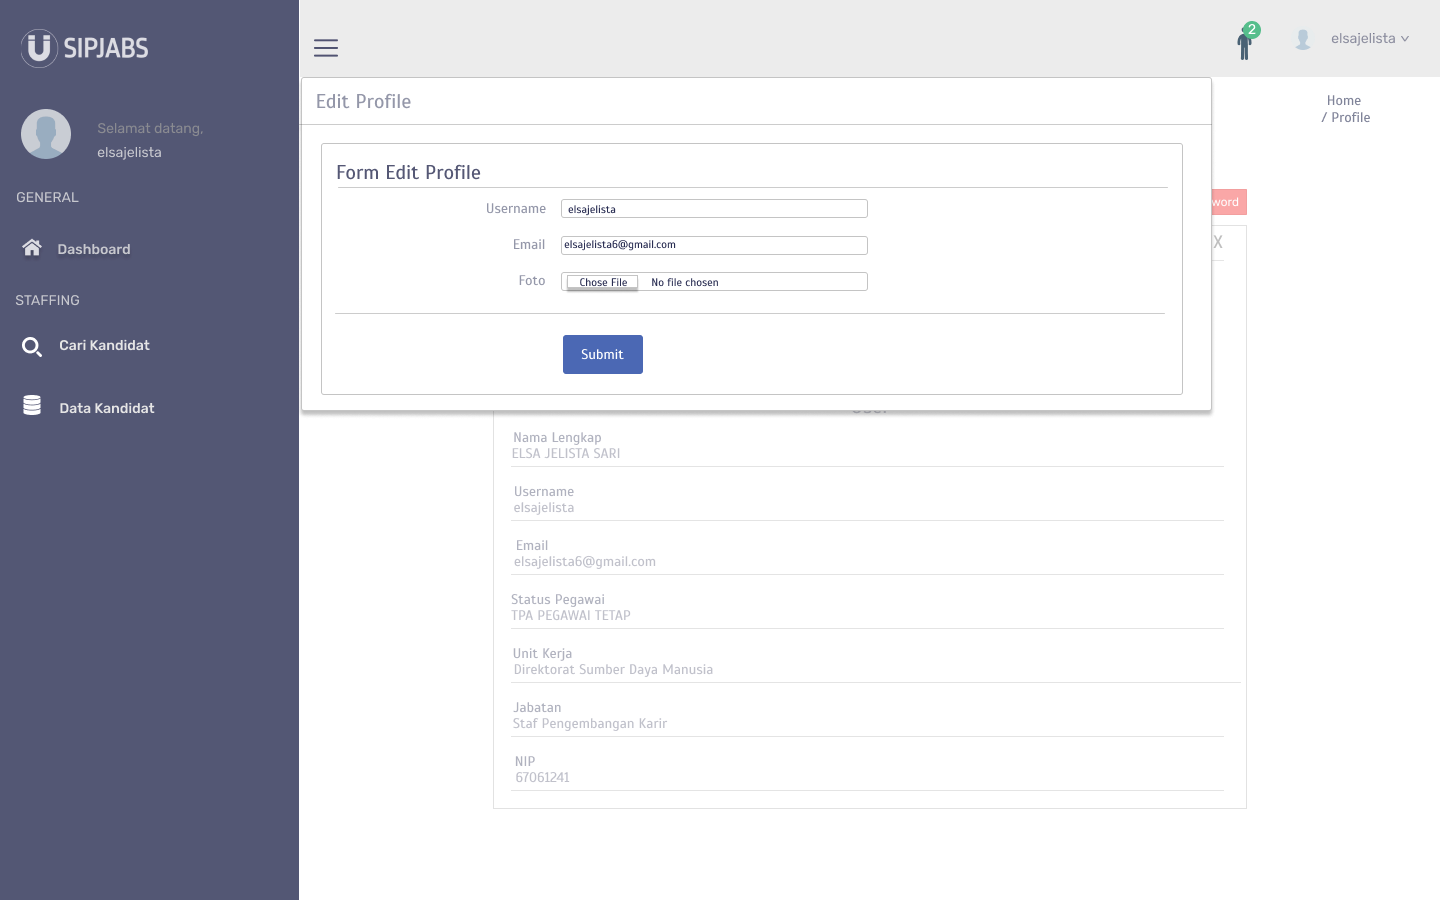
\includegraphics[width=0.6\textwidth, height=60mm]{pics/user/editprofile.png}} 
		& User dapat mengubah username, menginputkan email, dan menambahkan foto profile  \\
		
		\hline
		
		5. & \raisebox{-\totalheight}{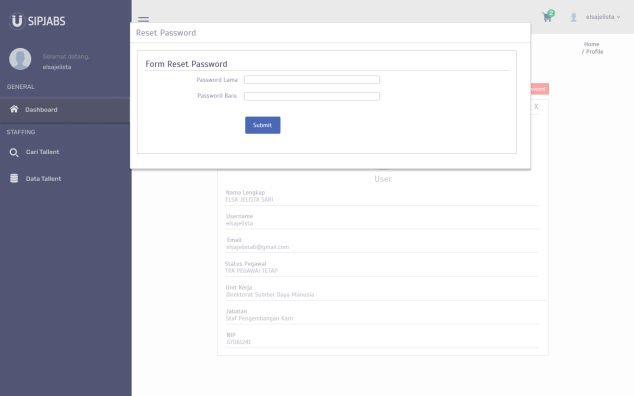
\includegraphics[width=0.6\textwidth, height=60mm]{pics/user/resetpassword.png}} 
		& User harus menginputkan password yang lama serta yang baru, setelah itu user dapat menyimpan.  \\
		
		\hline
		
		6. & \raisebox{-\totalheight}{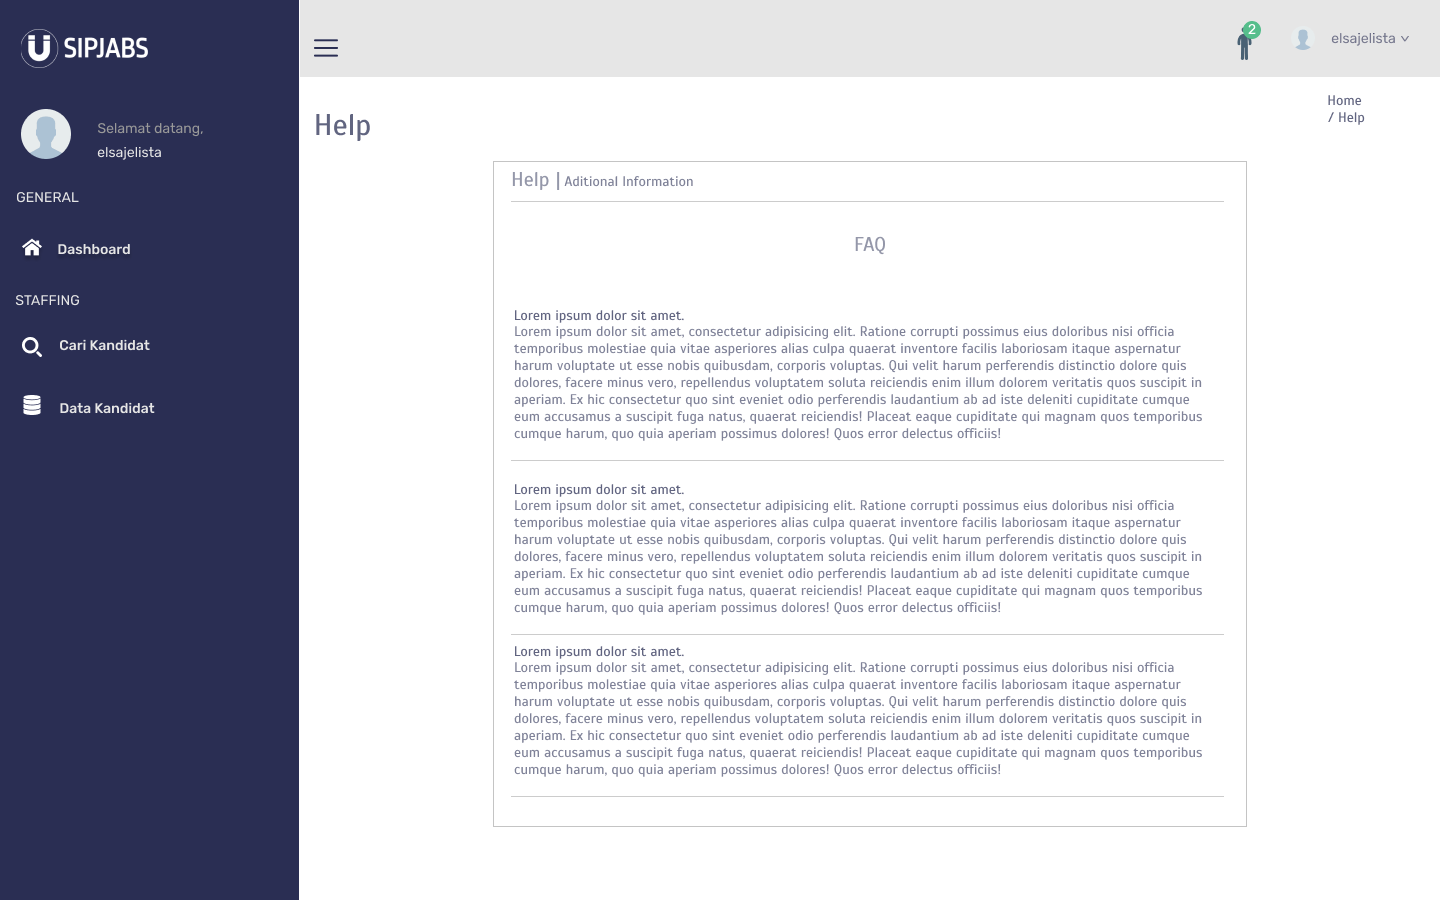
\includegraphics[width=0.6\textwidth, height=60mm]{pics/user/help.png}} 
		& Pada halaman help akan mengenai informasi dari sistem aplikasi ini\\
		
		\hline
		
	\end{tabular}
\end{table}

\begin{table}
	\caption{Tabel Perancangan Antar Muka User (2)}
	\centering
	\begin{tabular}{ | c | c | p{35mm} |}
		\hline 
		\textbf{No} & \textbf{Gambar} &  \textbf{Keterangan} \\ 
		\hline
		
		7. & \raisebox{-\totalheight}{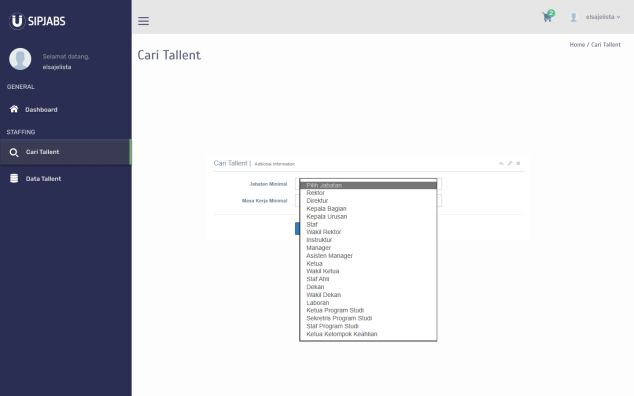
\includegraphics[width=0.6\textwidth, height=60mm]{pics/user/caritallent.png}} 
		& User dapat memilih jabatan dan masa kerja yang diinginkan untuk mengantikan atau mengisi posisi yang kosong.  \\
		
		\hline
		
		8. & \raisebox{-\totalheight}{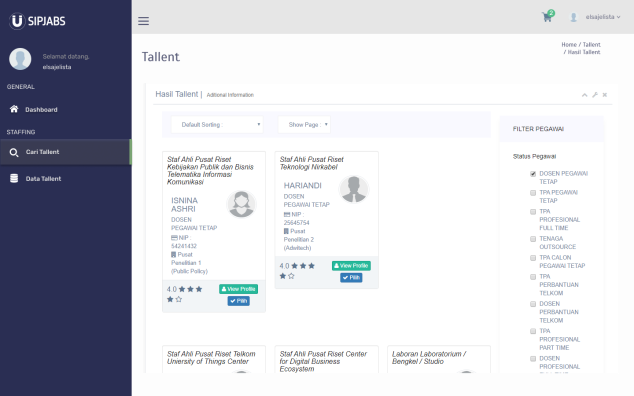
\includegraphics[width=0.6\textwidth, height=60mm]{pics/user/hasiltallent.png}} 
		& Halaman ini akan menampilkan tallent yang sudah di pilih dengan syarat tententu.   \\
		
		\hline
		
		9. & \raisebox{-\totalheight}{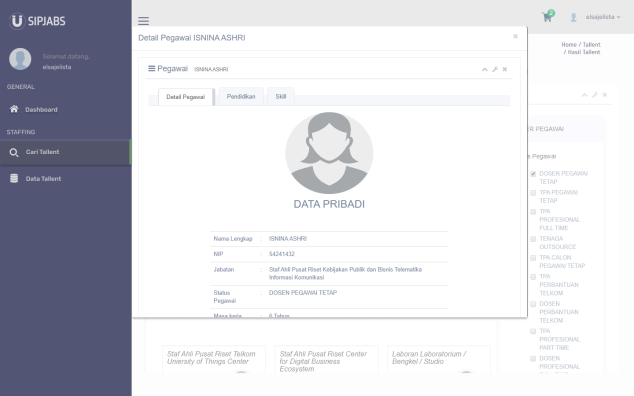
\includegraphics[width=0.6\textwidth, height=60mm]{pics/user/viewdetailtallent.png}} 
		& Halaman ini akan menampilkan data pribadi dari tallent tersebut.\\
		
		\hline
		
	\end{tabular}
\end{table}

\begin{table}
	\caption{Tabel Perancangan Antar Muka User (3)}
	\centering
	\begin{tabular}{ | c | c | p{35mm} |}
		\hline 
		\textbf{No} & \textbf{Gambar} &  \textbf{Keterangan} \\ 
		\hline
		
		10. & \raisebox{-\totalheight}{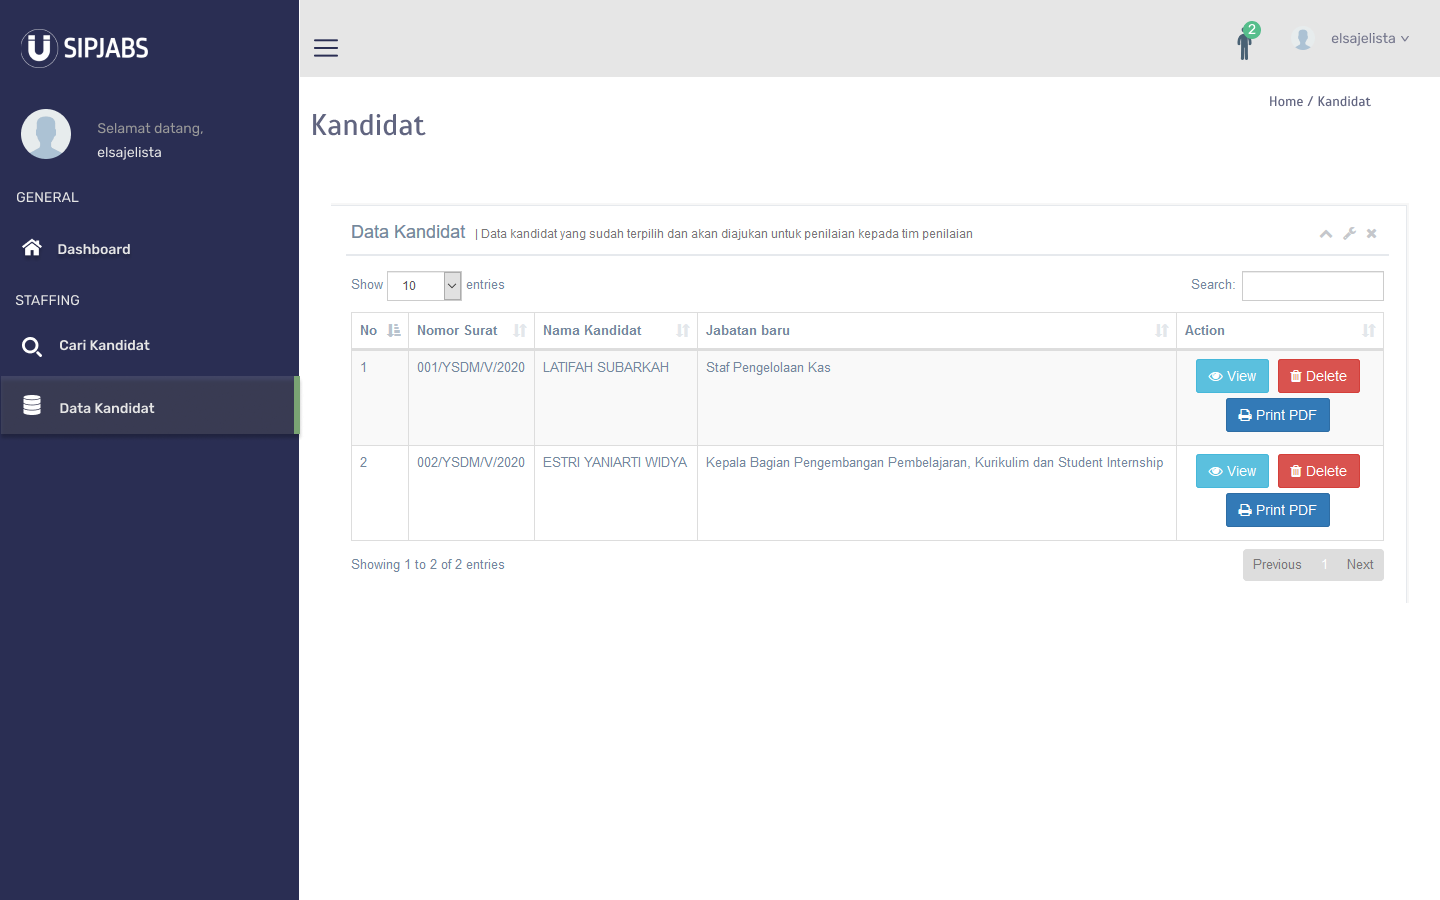
\includegraphics[width=0.6\textwidth, height=60mm]{pics/user/datatallent.png}} 
		& Halaman ini akan menampilkan data tallent yang sudah di proses dari cart tersebut.  \\
		
	
		\hline
		
		11. & \raisebox{-\totalheight}{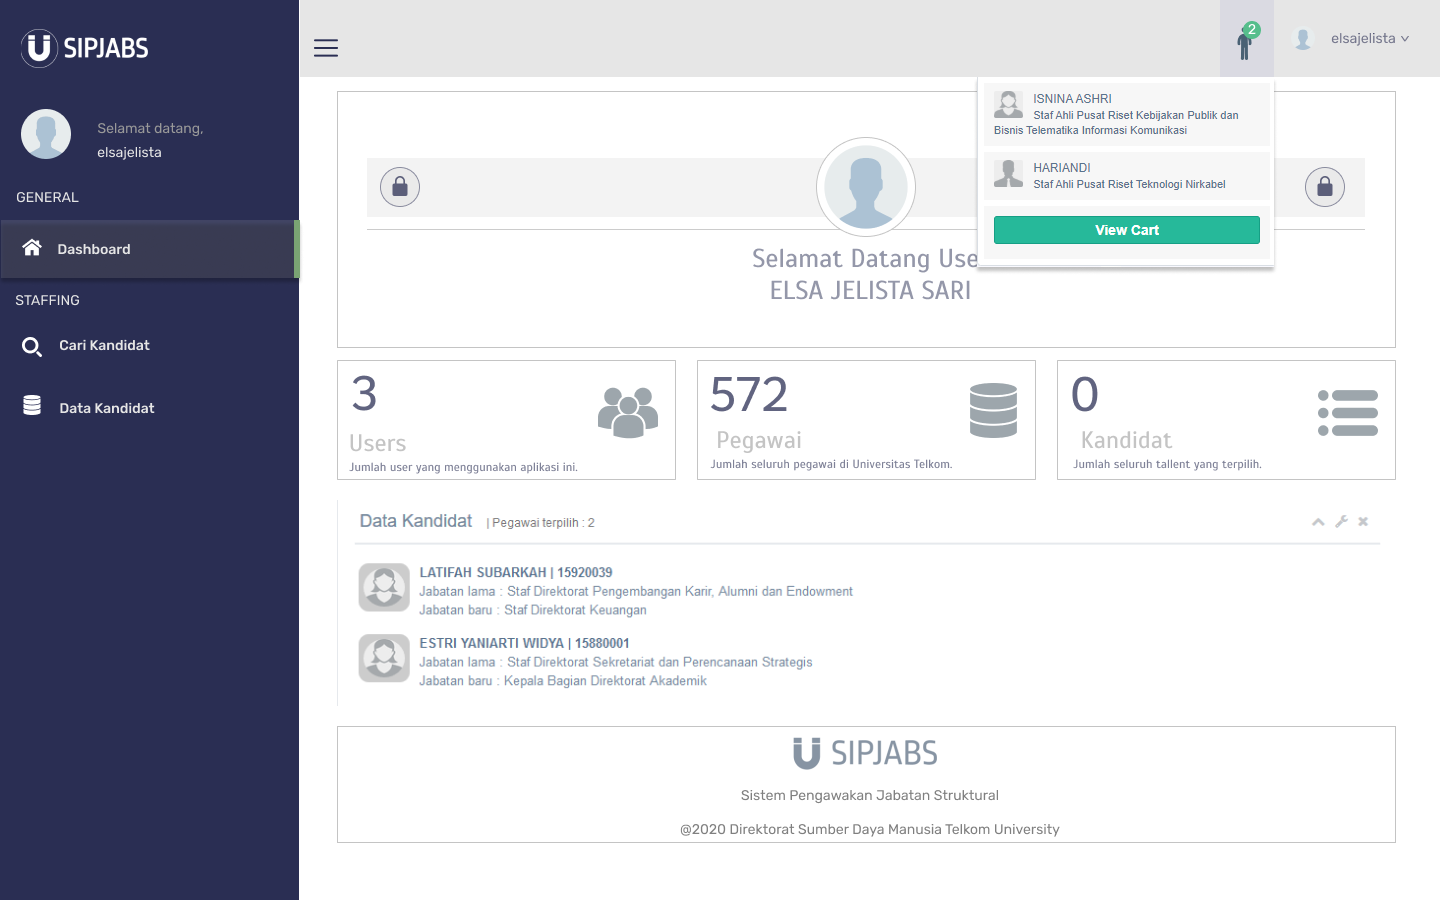
\includegraphics[width=0.6\textwidth, height=60mm]{pics/user/cartuser.png}} 
		& Halaman ini akan menampilkan data tallent yang sudah dipilih dan masih ada kemungkinan bisa di ubah sebelum ditetapkan menjadi tallent.  \\
		
		\hline
		
		12. & \raisebox{-\totalheight}{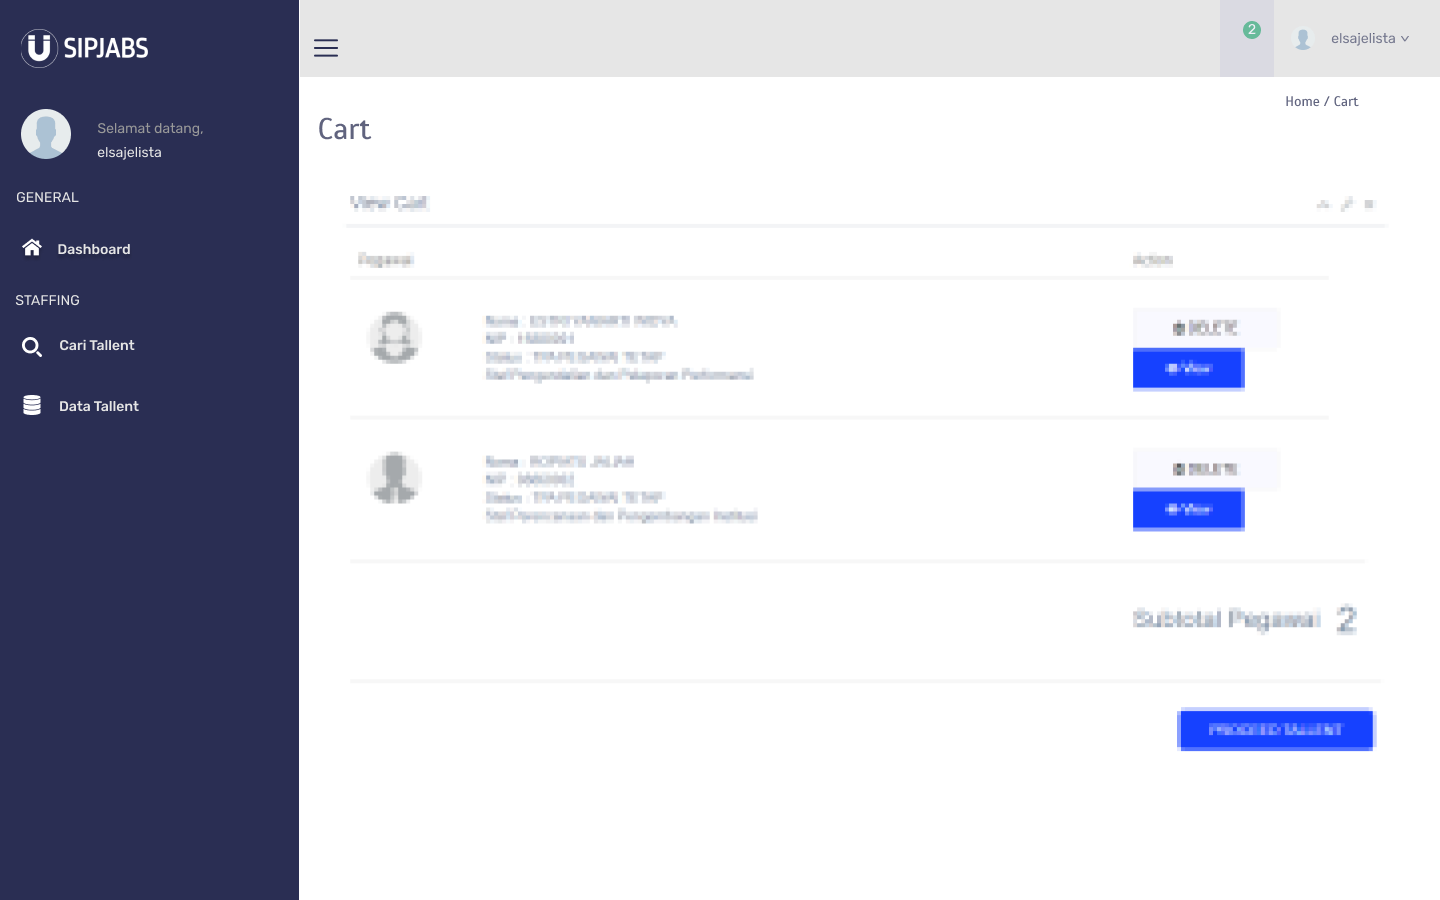
\includegraphics[width=0.6\textwidth, height=60mm]{pics/user/viewcart.png}} 
		& Halaman ini akan menampilkan data tallent yang sudah di pilih dan akan di proses ditetapkan untuk menjadi tallent.  \\
		
		
		\hline
		
	\end{tabular}
\end{table}
\subsection{Perancangan Level Tinggi}

\begin{figure}
	\centering
	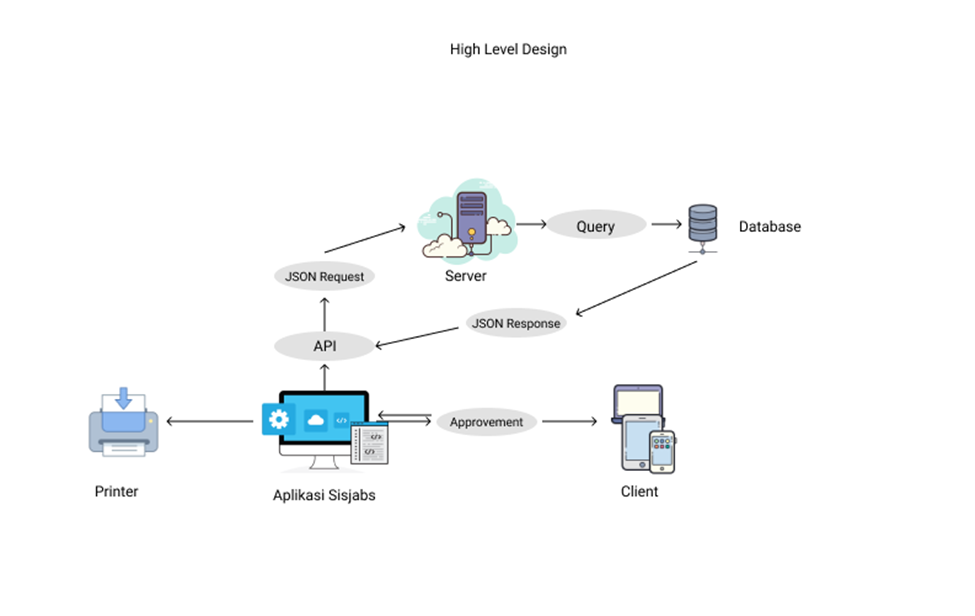
\includegraphics[width=0.9\textwidth]
	{pics/highleveldesign.png}
	\caption{High Level Design}
	\label{fig:34}
\end{figure}

Alur perancanaan level tinggi pada aplikasi pengawakan pegawai dimulai dari pengambilan API dalam bentuk JSON Request ke server. Pengambilan data akan di filter berdasarkan dengan query yang dibuat berdasarkan data yang diperoleh dari database yang ada. Kemudian database akan memberikan umpan balik berupa JSON Response berdasarkan request data yang akan ditampilkan kepada pengguna. 

